\documentclass[10pt,a4paper]{article}

\usepackage[T1]{fontenc}
\usepackage[utf8]{inputenc}
\usepackage{lmodern}
\usepackage[margin=2.3cm]{geometry}
\usepackage{amsmath,amssymb}
\usepackage{graphicx}
\usepackage{booktabs}
\usepackage{array}
\usepackage{url}
\usepackage{xcolor}
\usepackage{microtype}
\usepackage{siunitx}
\usepackage{algorithm}
\usepackage{algpseudocode}
\usepackage[hidelinks]{hyperref}
\usepackage{orcidlink}
\usepackage{caption}
\captionsetup{font=small,labelfont=bf}
\setlength{\parskip}{0.4em}
\setlength{\parindent}{0pt}
\sloppy

\graphicspath{{../figures/}}
% Written by data/measure.py: do not edit.
\newcommand{\parNens}{200}
\newcommand{\parEnsSeed}{999}
\newcommand{\parIters}{40}
\newcommand{\parWarm}{30}
\newcommand{\parAb}{0.02}
\newcommand{\parAbSqrt}{0.057}
\newcommand{\parAbRms}{0.057}
\newcommand{\parLevel}{0.90}
\newcommand{\parQ}{8}
\newcommand{\parLr}{0.02}
\newcommand{\workersUsed}{14}
\newcommand{\parCurvDelta}{0.05}
\newcommand{\nSeedsAll}{10}
\newcommand{\nSeedsThree}{3}
\newcommand{\ratioMed}{1.435}
\newcommand{\ratioMin}{1.42}
\newcommand{\ratioMax}{1.57}
\newcommand{\effRatioMed}{0.982}
\newcommand{\effRatioMin}{0.981}
\newcommand{\effRatioMax}{0.983}
\newcommand{\ratioAllMed}{1.439}
\newcommand{\ratioAllMin}{1.35}
\newcommand{\ratioAllMax}{1.57}
\newcommand{\ratioAllCiLo}{1.38}
\newcommand{\ratioAllCiHi}{1.48}
\newcommand{\effAllMed}{0.982}
\newcommand{\effAllMin}{0.981}
\newcommand{\effAllMax}{0.983}
\newcommand{\seedsPassing}{10}
\newcommand{\ciBelowN}{2}
\newcommand{\seedsEffPassing}{10}
\newcommand{\sigmaNomOne}{6.192}
\newcommand{\sigmaBfourOne}{3.947}
\newcommand{\ratioOne}{1.57}
\newcommand{\ratioOneLo}{1.34}
\newcommand{\ratioOneHi}{1.73}
\newcommand{\winsOne}{200}
\newcommand{\signPOne}{1.2\times10^{-60}}
\newcommand{\runSeconds}{115}
\newcommand{\totalMinutes}{15}
\newcommand{\pointonlyMinutes}{6}
\newcommand{\pointonlyWorkers}{3}
\newcommand{\evalMeanNom}{3.75}
\newcommand{\evalMeanBfour}{2.19}
\newcommand{\evalMaxNom}{10.4}
\newcommand{\evalMaxBfour}{7.6}
\newcommand{\evalMedNom}{3.63}
\newcommand{\evalMedBfour}{1.98}
\newcommand{\meanRatioOne}{1.71}
\newcommand{\levelAbs}{0.7125}
\newcommand{\effDropOne}{0.907}
\newcommand{\strehlExp}{0.881}
\newcommand{\phaseRms}{0.36}
\newcommand{\strehlThree}{0.75}
\newcommand{\startEffOne}{0.792}
\newcommand{\replicaDiff}{9.6e-13}
\newcommand{\evalCheckMax}{1.1e-14}
\newcommand{\lossStart}{0.00187}
\newcommand{\lossEnd}{0.000743}
\newcommand{\nIterHist}{40}
\newcommand{\heldMed}{1.58}
\newcommand{\heldMin}{1.47}
\newcommand{\heldMax}{1.79}
\newcommand{\heldN}{15}
\newcommand{\heldEffMed}{0.982}
\newcommand{\misAMed}{1.24}
\newcommand{\misAMin}{1.22}
\newcommand{\misAMax}{1.34}
\newcommand{\misBMed}{1.75}
\newcommand{\misBMin}{1.72}
\newcommand{\misBMax}{1.77}
\newcommand{\misCMed}{1.43}
\newcommand{\misCMin}{1.42}
\newcommand{\misCMax}{1.57}
\newcommand{\misDMed}{1.16}
\newcommand{\misDMin}{1.06}
\newcommand{\misDMax}{1.20}
\newcommand{\misEMed}{1.02}
\newcommand{\misEMin}{0.99}
\newcommand{\misEMax}{1.03}
\newcommand{\misFMed}{1.22}
\newcommand{\misFMin}{1.19}
\newcommand{\misFMax}{1.24}
\newcommand{\misGMed}{0.99}
\newcommand{\misGMin}{0.97}
\newcommand{\misGMax}{1.02}
\newcommand{\thPearsonNom}{0.978}
\newcommand{\thPtotalNom}{8.5e-06}
\newcommand{\thMeasSqNom}{14.87}
\newcommand{\thPredSqNom}{13.59}
\newcommand{\thBoundSqNom}{13.59}
\newcommand{\thQMeasNom}{6.07}
\newcommand{\thQLinNom}{5.70}
\newcommand{\thSigmaZeroNom}{0.015}
\newcommand{\thDeltaJNom}{$-$0.0105}
\newcommand{\thGNNom}{0.00166}
\newcommand{\thLzeroNom}{0.0123}
\newcommand{\thJsigNom}{0.00185}
\newcommand{\thPearsonBfour}{0.877}
\newcommand{\thPtotalBfour}{1.72e-06}
\newcommand{\thMeasSqBfour}{5.66}
\newcommand{\thPredSqBfour}{3.81}
\newcommand{\thBoundSqBfour}{3.82}
\newcommand{\thQMeasBfour}{4.22}
\newcommand{\thQLinBfour}{2.79}
\newcommand{\thSigmaZeroBfour}{1}
\newcommand{\thDeltaJBfour}{$-$0.00758}
\newcommand{\thGNBfour}{0.000336}
\newcommand{\thLzeroBfour}{0.00824}
\newcommand{\thJsigBfour}{0.000669}
\newcommand{\thPRatio}{4.92}
\newcommand{\thQLinRatio}{2.04}
\newcommand{\thResidNom}{$-$0.012}
\newcommand{\ptAccMed}{1.04}
\newcommand{\ptAccMin}{0.85}
\newcommand{\ptAccMax}{1.05}
\newcommand{\ptAccOne}{1.04}
\newcommand{\ptAccNomOne}{8.492}
\newcommand{\ptAccBfourOne}{8.152}
\newcommand{\ptASample}{1.06}
\newcommand{\ptASampleMin}{1.06}
\newcommand{\ptASampleMax}{1.12}
\newcommand{\ptASigma}{1.29}
\newcommand{\ptAEff}{0.997}
\newcommand{\ptBSample}{1.07}
\newcommand{\ptBSampleMin}{1.05}
\newcommand{\ptBSampleMax}{1.08}
\newcommand{\ptBSigma}{1.26}
\newcommand{\ptBEff}{0.998}
\newcommand{\ptCSample}{1.02}
\newcommand{\ptCSampleMin}{1.02}
\newcommand{\ptCSampleMax}{1.03}
\newcommand{\ptCSigma}{1.14}
\newcommand{\ptCEff}{0.998}
\newcommand{\curvNom}{1.231}
\newcommand{\curvBfour}{1.227}
\newcommand{\curvAp}{1.252}
\newcommand{\curvRelLoss}{1.4}
\newcommand{\poANom}{1.09}
\newcommand{\poAPred}{0.31}
\newcommand{\poAPredSlope}{1.06}
\newcommand{\poABfour}{1.49}
\newcommand{\poADesign}{1.52}
\newcommand{\poARatio}{0.74}
\newcommand{\poARatioMin}{0.69}
\newcommand{\poARatioMax}{0.81}
\newcommand{\poAEff}{0.963}
\newcommand{\poBNom}{2.33}
\newcommand{\poBPred}{1.23}
\newcommand{\poBPredSlope}{2.38}
\newcommand{\poBBfour}{2.61}
\newcommand{\poBDesign}{2.45}
\newcommand{\poBRatio}{1.01}
\newcommand{\poBRatioMin}{0.94}
\newcommand{\poBRatioMax}{1.01}
\newcommand{\poBEff}{0.976}
\newcommand{\poCNom}{3.98}
\newcommand{\poCPred}{2.77}
\newcommand{\poCPredSlope}{4.12}
\newcommand{\poCBfour}{4.19}
\newcommand{\poCDesign}{3.82}
\newcommand{\poCRatio}{1.07}
\newcommand{\poCRatioMin}{1.03}
\newcommand{\poCRatioMax}{1.07}
\newcommand{\poCEff}{0.984}
\newcommand{\poALong}{1.11}
\newcommand{\poALongMin}{1.02}
\newcommand{\poALongMax}{1.24}
\newcommand{\poALongEff}{0.902}
\newcommand{\poALongMean}{0.98}
\newcommand{\poALongSlope}{0.027}
\newcommand{\poALongCurv}{1.229}
\newcommand{\poBLong}{1.48}
\newcommand{\poBLongMin}{1.44}
\newcommand{\poBLongMax}{1.50}
\newcommand{\poBLongEff}{0.912}
\newcommand{\poBLongMean}{1.60}
\newcommand{\poBLongSlope}{0.009}
\newcommand{\poBLongCurv}{1.221}
\newcommand{\poCLong}{1.37}
\newcommand{\poCLongMin}{1.36}
\newcommand{\poCLongMax}{1.43}
\newcommand{\poCLongEff}{0.923}
\newcommand{\poCLongMean}{2.86}
\newcommand{\poCLongSlope}{0.003}
\newcommand{\poCLongCurv}{1.212}
\newcommand{\poKx}{1.231}
\newcommand{\poKy}{1.232}
\newcommand{\poSlopeSq}{0.041}
\newcommand{\poSlopeRms}{0.20}
\newcommand{\poSlopeSqBfour}{0.046}
\newcommand{\ablNominalMed}{0.62}
\newcommand{\ablNominalMin}{0.56}
\newcommand{\ablNominalMax}{0.71}
\newcommand{\ablNominalEff}{0.891}
\newcommand{\ablRandFourMed}{1.00}
\newcommand{\ablRandFourMin}{0.98}
\newcommand{\ablRandFourMax}{1.12}
\newcommand{\ablRandFourEff}{0.952}
\newcommand{\ablRandEightMed}{1.20}
\newcommand{\ablRandEightMin}{1.12}
\newcommand{\ablRandEightMax}{1.21}
\newcommand{\ablRandEightEff}{0.972}
\newcommand{\ablRandSixteenMed}{1.33}
\newcommand{\ablRandSixteenMin}{1.26}
\newcommand{\ablRandSixteenMax}{1.36}
\newcommand{\ablRandSixteenEff}{0.974}
\newcommand{\ablRandThirtyTwoMed}{1.39}
\newcommand{\ablRandThirtyTwoMin}{1.33}
\newcommand{\ablRandThirtyTwoMax}{1.44}
\newcommand{\ablRandThirtyTwoEff}{0.980}
\newcommand{\ablAdamMed}{1.24}
\newcommand{\ablAdamMin}{1.16}
\newcommand{\ablAdamMax}{1.28}
\newcommand{\ablAdamEff}{0.988}
\newcommand{\ablModesDefocusMed}{0.75}
\newcommand{\ablModesDefocusMin}{0.59}
\newcommand{\ablModesDefocusMax}{0.82}
\newcommand{\ablModesDefocusEff}{0.901}
\newcommand{\ablModesToSixMed}{0.92}
\newcommand{\ablModesToSixMin}{0.70}
\newcommand{\ablModesToSixMax}{0.92}
\newcommand{\ablModesToSixEff}{0.924}
\newcommand{\ablModesToEightMed}{1.17}
\newcommand{\ablModesToEightMin}{1.13}
\newcommand{\ablModesToEightMax}{1.17}
\newcommand{\ablModesToEightEff}{0.952}
\newcommand{\ablModesHighMed}{0.89}
\newcommand{\ablModesHighMin}{0.75}
\newcommand{\ablModesHighMax}{0.94}
\newcommand{\ablModesHighEff}{0.924}
\newcommand{\ablPriorAMed}{0.65}
\newcommand{\ablPriorAMin}{0.60}
\newcommand{\ablPriorAMax}{0.75}
\newcommand{\ablPriorAEff}{0.898}
\newcommand{\ablPriorBMed}{0.84}
\newcommand{\ablPriorBMin}{0.83}
\newcommand{\ablPriorBMax}{0.87}
\newcommand{\ablPriorBEff}{0.916}
\newcommand{\ablPriorDMed}{1.13}
\newcommand{\ablPriorDMin}{1.07}
\newcommand{\ablPriorDMax}{1.23}
\newcommand{\ablPriorDEff}{1.012}
\newcommand{\ablPriorEMed}{0.90}
\newcommand{\ablPriorEMin}{0.90}
\newcommand{\ablPriorEMax}{0.98}
\newcommand{\ablPriorEEff}{1.016}
\newcommand{\ablLevelAMed}{0.71}
\newcommand{\ablLevelAMin}{0.53}
\newcommand{\ablLevelAMax}{0.78}
\newcommand{\ablLevelAEff}{0.849}
\newcommand{\ablLevelBMed}{1.25}
\newcommand{\ablLevelBMin}{1.04}
\newcommand{\ablLevelBMax}{1.29}
\newcommand{\ablLevelBEff}{0.929}
\newcommand{\ablLevelDMed}{1.27}
\newcommand{\ablLevelDMin}{1.24}
\newcommand{\ablLevelDMax}{1.33}
\newcommand{\ablLevelDEff}{1.006}
\newcommand{\ablLevelEMed}{1.19}
\newcommand{\ablLevelEMin}{1.18}
\newcommand{\ablLevelEMax}{1.26}
\newcommand{\ablLevelEEff}{1.009}
\newcommand{\ablLevelFMed}{1.06}
\newcommand{\ablLevelFMin}{1.04}
\newcommand{\ablLevelFMax}{1.14}
\newcommand{\ablLevelFEff}{1.014}
\newcommand{\ablIterAMed}{1.30}
\newcommand{\ablIterAMin}{1.28}
\newcommand{\ablIterAMax}{1.36}
\newcommand{\ablIterAEff}{0.981}
\newcommand{\ablIterBMed}{1.33}
\newcommand{\ablIterBMin}{1.27}
\newcommand{\ablIterBMax}{1.37}
\newcommand{\ablIterBEff}{0.978}
\newcommand{\ablIterCMed}{1.40}
\newcommand{\ablIterCMin}{1.39}
\newcommand{\ablIterCMax}{1.53}
\newcommand{\ablIterCEff}{0.981}
\newcommand{\ablIterEMed}{1.44}
\newcommand{\ablIterEMin}{1.42}
\newcommand{\ablIterEMax}{1.56}
\newcommand{\ablIterEEff}{0.984}
\newcommand{\ablDefaultMed}{1.43}
\newcommand{\ablDefaultMin}{1.42}
\newcommand{\ablDefaultMax}{1.57}
\newcommand{\ablDefaultEff}{0.982}
\newcommand{\pubGSPn}{19.25}
\newcommand{\pubGSRatio}{0.31}
\newcommand{\pubGSEff}{1.025}
\newcommand{\pubGAAPn}{14.55}
\newcommand{\pubGAARatio}{0.42}
\newcommand{\pubGAAEff}{1.021}
\newcommand{\pubGSWPn}{6.06}
\newcommand{\pubGSWRatio}{1.00}
\newcommand{\pubGSWEff}{1.015}
\newcommand{\pubPFWGSPn}{6.07}
\newcommand{\pubPFWGSRatio}{1.00}
\newcommand{\pubPFWGSEff}{1.000}
\newcommand{\pubCGPn}{35.16}
\newcommand{\pubCGRatio}{0.17}
\newcommand{\pubCGEff}{0.371}
\newcommand{\pubWirtPn}{6.34}
\newcommand{\pubWirtRatio}{0.96}
\newcommand{\pubWirtEff}{0.994}
\newcommand{\pubBfourPn}{4.22}
\newcommand{\pubBfourRatio}{1.43}
\newcommand{\pubBfourEff}{0.982}
\newcommand{\bakeIdealBelow}{6}
\newcommand{\bakeIdealN}{9}
\newcommand{\bakeNineB}{5.31}
\newcommand{\bakeNineM}{6.16}
\newcommand{\bakeNineRatio}{1.16}
\newcommand{\bakeNineEff}{0.99}


% Page-1 header block (conventions/manuscript-header-standard.md). The four document macros are set by the
% publishing tool when the version DOI is reserved.
\newcommand{\doctype}{Preprint}
\newcommand{\docversion}{v0.01}
\newcommand{\docdate}{3 November 2026}
\newcommand{\versiondoi}{10.5281/zenodo.pending}
\newcommand{\conceptdoi}{10.5281/zenodo.pending}
\newcommand{\docrepo}{github.com/fsantibanezleal/CEFOP\_DinHot}
\newcommand{\headerblock}{%
\begin{center}
\fbox{\parbox{0.94\textwidth}{\small\raggedright
\textbf{\doctype} \quad$\cdot$\quad \docversion, \docdate \quad$\cdot$\quad Licence CC BY 4.0\\[2pt]
CAOS open-research programme \quad$\cdot$\quad CEFOP\_DinHot, holographic optical trap studio\\[2pt]
Version DOI \href{https://doi.org/\versiondoi}{\texttt{\versiondoi}} \quad$\cdot$\quad
concept DOI (always latest) \href{https://doi.org/\conceptdoi}{\texttt{\conceptdoi}}\\[2pt]
Not peer reviewed. Source code, data and computational records: \href{https://\docrepo}{\texttt{\docrepo}}
}}
\end{center}
\vspace{4pt}}

\begin{document}

\title{Aberration-Robust Holograms for Optical Trap Arrays: Expected-Cost Optimization Lowers the Tail of the Intensity Spread Under Residual Aberrations Drawn from Its Design Prior, in Simulation}
\author{Felipe Santib\'a\~nez-Leal~\orcidlink{0000-0002-0150-3246}\\
\small CAOS open-research programme, Santiago, Chile\\
\small \texttt{fsantibanez@gmail.com}}
\date{}
\maketitle
\vspace{-1.2em}
\headerblock

\begin{abstract}
Weighted Gerchberg--Saxton holograms equalize the traps of an optical tweezer array for the nominal optical system, and the aberrations that remain after a wavefront correction then change the trap intensities in ways the hologram was never asked to resist. We minimize the expected trap-intensity cost over a Gaussian prior on residual Zernike aberrations (Noll 4 to 11), replace the expectation by sixteen sigma points so that a conjugate-gradient descent from phase-fixed weighted Gerchberg--Saxton sees a noise-free cost with a closed-form gradient, and derive that the sigma points match the expectation through second order and that the robust cost adds the first-order intensity variance that the aberrations induce. On a $10\times10$ array in a scalar Fourier model, over an ensemble of \parNens{} draws of \parAb{} waves per mode, the 95th percentile of the relative standard deviation of the trap intensities is a median of \ratioMed{} times lower than for phase-fixed weighted Gerchberg--Saxton (\ratioMin{} to \ratioMax{} over three seeds; \ratioAllMed{} over \nSeedsAll{} seeds, interval \ratioAllCiLo{} to \ratioAllCiHi) at \effRatioMed{} of its efficiency. The same solver on the nominal cost gives \ablNominalMed, so the expected cost causes the gain; sixteen random draws give \ablRandSixteenMed. The gain falls to \misEMed{} at twice the design amplitude and \misGMed{} when modes outside the design are present, the first-order model overstates the gain, and for random displacements of the traps the acceptance configuration gives \ptAccMed{}, while a displacement prior optimized alone for 100 steps gives \poBLong{} at 0.10 focal bins at \poBLongEff{} of the efficiency. The results are simulations without pixel crosstalk and not hardware measurements.
\end{abstract}

\noindent\textbf{Keywords:} holographic optical tweezers, weighted Gerchberg--Saxton, residual aberrations, expected-cost optimization, sigma points, Zernike polynomials.


\section{Introduction}\label{sec:intro}

A phase-only spatial light modulator (SLM) in the pupil plane of a lens turns a computed phase pattern into an array of optical traps. The first single-beam gradient-force trap
demonstrated that a focused beam holds a dielectric particle~\cite{ashkin1986}; the holograms that make hundreds or thousands of such traps from one beam are computed, not designed, by
iterative Fourier algorithms whose weighted form equalizes the trap intensities~\cite{dileonardo2007}. The same computation now sets the size of neutral-atom quantum machines. The
256-atom simulator of Ebadi et al.\ computes its holograms with phase-fixed weighted Gerchberg--Saxton (WGS) for roughly one thousand tweezers and corrects the aberrations of the optics with
Zernike polynomials set on the SLM~\cite{ebadi2021}; the array of Manetsch et al.\ holds 6,100 atoms in 11,998 sites and still shows a standard deviation of the trap depth across sites of 11.4
percent after the WGS optimization, and the authors report that optical aberrations worsen at tweezer powers above the ones they used~\cite{manetsch2025}. The light field, not the
atom physics, is a limit of the machine, and aberrations are one named part of that limit.

The established remedy for an aberrated optical train is to measure the wavefront and display its opposite on the SLM. Nogrette et al.\ added the aberration phase to the hologram phase and
reduced the root-mean-square (rms) wavefront error from 0.15 to 0.014 wavelengths, which raised the radial trap frequency from 68.0 to 86.5 kHz~\cite{nogrette2014}. A correction is a point estimate,
however. The aberration of a tweezer array depends on the position in the field: a modified Gerchberg--Saxton algorithm that uses aberrations measured over the whole field extends the aberration-free
field of view from 50 to 500 micrometres~\cite{machu2025}, and per-site propagation kernels grouped into about 50 isoplanatic patches enlarge the field of view of a tweezer array eightfold~\cite{christen2025}.
Whatever the correction, a residual remains, it differs from site to site and from one calibration to the next, and the hologram that was optimized for the nominal system meets it unprepared. A hologram
can be made less sensitive to what the correction leaves; the sources read for this paper correct the aberration per site or with one global set, and none optimizes the hologram for a distribution of residual
aberration.

We propose that distribution-level design and test it. The aberration-robust hologram minimizes the expected trap-intensity loss over a prior on the residual Zernike coefficients, instead of the loss at the
nominal system. The expectation is taken by a deterministic set of sigma points, which gives the optimizer a cost without sampling noise, and the minimization is a conjugate-gradient descent started from the
hologram of phase-fixed WGS, the method that computes the holograms of the largest arrays. The method is not a new optimizer: it is a choice of the cost that a gradient method minimizes, a derivation of why that cost
lowers the spread of the trap intensities under aberration, and a measurement of where it helps and where it does not.

The contributions are the following.
\begin{enumerate}
\item A formulation of the hologram design as the minimization of the expected loss over residual aberrations, with a sigma-point quadrature that matches the Gaussian expectation through the second order in the prior
standard deviation, and a closed-form gradient (Sections~\ref{sec:problem} and~\ref{sec:proposed-method}).
\item Three propositions with derivations: the accuracy of the sigma-point quadrature, the decomposition of the robust cost into the nominal cost plus a curvature term along the aberration modes, and a bound of the
expected squared intensity spread by the Gauss--Newton part of that term; and a derived and measured limit, the curvature of a trap spot, that bounds what a design can gain under displacements of the traps
(Section~\ref{sec:theory}).
\item A measurement against the published methods run by the product on the same task and the same ensemble of 200 aberration draws, over \nSeedsAll{} seeds of the hologram, with bootstrap intervals, a paired sign test
and a check of the first-order theory against the ensemble (Sections~\ref{sec:design} and~\ref{sec:results}).
\item An ablation of the number and kind of design samples, the modes in the design, the design amplitude, the target level and the iterations, and a test on ensembles that differ from the design prior
(Sections~\ref{sec:results} and~\ref{sec:ablation}).
\end{enumerate}

The main result is a spread result in a simulated device and not a hardware measurement. Over an ensemble of 200 draws of eight residual Zernike modes (Noll 4 to 11) of \parAb{} waves standard deviation each, the 95th percentile of the
relative standard deviation of the trap intensities of a $10\times10$ array is a median of \ratioMed{} times lower for the robust hologram than for phase-fixed WGS (\ratioMin{} to \ratioMax{} over three seeds of the holograms; median
\ratioAllMed{} over \nSeedsAll{} seeds, bootstrap interval \ratioAllCiLo{} to \ratioAllCiHi), at a median \effRatioMed{} of the efficiency of phase-fixed WGS. The gain does not follow for random displacements of the traps in the configuration of the acceptance test: the same cost
extended with a displacement prior gives \ptAccMed{} times (\ptAccMin{} to \ptAccMax) and at most \ptASampleMax{} times with 20 steps (Table~\ref{tab:pointing}). With a displacement prior alone and five times the budget the ratio is \poBLong{} at 0.10 focal bins, at \poBLongEff{} of the efficiency, and we show that the spread under displacement has a first-order
slope term, which a design can lower, and a curvature floor, which the width of the focused spot fixes.

The paper is organized as follows. Section~\ref{sec:related} places the method among the published ones. Section~\ref{sec:problem} fixes the model, the metrics and the problem. Section~\ref{sec:proposed-method} derives the method and
gives its algorithm, parameters and cost. Section~\ref{sec:theory} states and proves what can be proved. Section~\ref{sec:design} states the hypotheses and the protocol, Section~\ref{sec:results} reports the measurements and
Section~\ref{sec:ablation} the ablation. Sections~\ref{sec:discussion} and~\ref{sec:limits} discuss the findings and the limits, Section~\ref{sec:repro} gives the commands that rebuild every number, and
Section~\ref{sec:conclusions} concludes.

\section{Related work}\label{sec:related}

\subsection{Hologram computation for trap arrays}

Three families of method compute the phase of an array of point traps. The first is direct: random-mask encoding multiplexes the phase-only filters of the single traps without iteration and is extremely fast, at the price of an
uneven result~\cite{montes2006}. The second is the Gerchberg--Saxton (GS) iteration and its weighted variants. Di Leonardo et al.\ replace the amplitudes in the trap plane by the target amplitudes and reweight them by the ratio of the mean to the
achieved amplitude, which equalizes the traps in the ideal model~\cite{dileonardo2007}; Kim et al.\ freeze the focal-plane phase after a few weighted iterations (phase-fixed WGS) so that the weights stay effective, and report 91.2 percent
efficiency with a non-uniformity below 0.5 percent on an array of $50\times30$ foci~\cite{kim2019}. The same procedure computes the holograms of the largest tweezer arrays~\cite{ebadi2021,manetsch2025}. The third family minimizes a cost.
Polin et al.\ search the phase of one pixel at a time~\cite{polin2005}; Pasienski and DeMarco free the amplitude outside a signal region so that the signal region is matched more closely~\cite{pasienski2008}; Harte et al.\ minimize a
power of the intensity error with conjugate gradients and remove the vortices that the basic cost leaves~\cite{harte2014}, and Bowman et al.\ extend the minimization to control phase and amplitude of the field together~\cite{bowman2017}.
All of them optimize the hologram for the nominal system: a perfect lens, an ideal SLM and a known beam.

\subsection{Gradient models of the optical path and learned generators}

When the cost is differentiable in the phase, any propagation model can be placed in the loop. Chakravarthula et al.\ derive Wirtinger gradients of a hologram loss and minimize it with the Adam optimizer~\cite{chakravarthula2019};
neural holography adds a calibrated model and a camera in the training loop~\cite{peng2020}. Learned generators trade the iteration for a network: a U-Net trained without labels on the plane images computes holograms of volumes~\cite{eybposh2020},
and a convolutional network of modest size computes three-dimensional holograms for displays~\cite{shi2021}; the three-dimensional extension of Gerchberg--Saxton propagates the field plane by plane~\cite{whyte2005}.
Schroff et al.\ place a crosstalk model of the SLM in a conjugate-gradient minimization with automatic differentiation, lower the error of shaped potentials and pay about ten minutes per hologram~\cite{schroff2023}, while Persson et al.\ modify a weighted
GS to account for pixel crosstalk~\cite{persson2012}. These works put a model of the device in the optimization; none puts a distribution of device or system states there.

\subsection{Aberrations of the optical train and their correction}

Aberrations are a long-standing limit of optical systems, and their treatment has two parts, measurement and compensation. Zernike polynomials are the usual basis to describe a wavefront; their general properties and the Zernike representation of
turbulence are given by Noll~\cite{noll1976}, and Mah\'ajan relates the Strehl ratio of circular and annular pupils to the variance of the phase aberration, finding the exponential of minus that variance a better approximation than the Mar\'echal formula~\cite{mahajan1983}.
Adaptive optics corrects aberrations in microscopy~\cite{booth2007}. For the SLM itself, the surface deviations are corrected from the shape of a single optical vortex created by the modulator~\cite{jesacher2007}, and an in situ wavefront
correction by complex modulation compensates the aberrations of the whole optical train for micromanipulation~\cite{cizmar2010}. In tweezer arrays the wavefront is measured and its opposite is added to the hologram phase~\cite{nogrette2014}, with
the same single Zernike set serving the whole array in the 256-atom and 6,100-atom machines~\cite{ebadi2021,manetsch2025}. Position-dependent aberrations are treated per site or per patch: a modified GS algorithm with aberrations measured over the full field~\cite{machu2025}, and per-site propagation
kernels combined in one hologram over about 50 isoplanatic patches with eight aberration modes~\cite{christen2025}.

\subsection{Rearrangement and moving traps, and the role of uniformity}

The need for uniform traps comes from the use of the arrays. A logical quantum processor on up to 280 physical qubits is built on reconfigurable atom arrays~\cite{bluvstein2023}, and such arrays are brought to a defect-free configuration by moving traps. An SLM-only approach for rearrangement uses
GS with zero padding and weighted feedback~\cite{kim2019oe}, and linear phase interpolation computes two endpoint WGS holograms and interpolates between them to keep the spot intensity above 70 percent while atoms move~\cite{knottnerus2025}.
In every one of these uses the trap depth varies with the intensity of the trap, so the spread of the intensities, and not only their mean, sets the quality of the array. The same holds for the loading of atoms into the traps and for the gates applied to them: a site that is dimmer than its neighbours is a site that differs from them. For the same reason the quantity that this paper controls is the spread of the intensities over the traps of one array, evaluated over the family of optical conditions that the array may meet, because an experiment runs its sequences in one of those conditions and not in the nominal one.

\subsection{Robust and stochastic optimization}

Minimizing the expectation of a cost over a random parameter is stochastic programming, and requiring the cost to hold over an uncertainty set is robust optimization; the latter is developed with its theory and applications by Ben-Tal et al.~\cite{bental2009}.
The expectation can be replaced by a small deterministic set of points, as the unscented transformation does to propagate a mean and a covariance through a nonlinear map~\cite{julier2004}; the optimizers used here are the Fletcher--Reeves nonlinear conjugate gradient~\cite{fletcher1964} with a strong-Wolfe line
search~\cite{nocedal2006}, and Adam~\cite{kingma2015} for the sampled variant. The choice between the two ways of taking the expectation is a choice between a smooth deterministic cost that a line search can use and a noisy cost that needs a stochastic optimizer; the second reaches any prior, including one that cannot be written as a phase offset (such as random displacements of the traps), and the first reaches the aberration prior with a few function evaluations per step. Both rely on the same property of the problem, that the forward map is a finite sum of complex exponentials of the phases, so that value and gradient of the cost at any perturbed system are closed forms that cost one forward and one adjoint evaluation of the point-trap model.

\subsection{Position of the proposed method}

Table~\ref{tab:related} lists the works that bound the gap with what each assumes and where it falls short for the task of this paper: uniform point traps whose intensities stay uniform when the optical system differs from the nominal one. The proposed
method takes the cost and the solver from the minimization family, the start from phase-fixed WGS, the Zernike basis and the additive aberration model from the correction literature, and the expectation from stochastic programming. Each piece is published; the
combination, the derivation of why the expected cost lowers the intensity spread, and the measurement of its scope are the contribution. The method is not an aberration correction: it takes no wavefront measurement, it leaves the correction in place and designs for what the
correction leaves.

\begin{table}[t]
\centering\small
\caption{Published methods that bound the gap: what each assumes and where it falls short for uniform point traps under residual aberrations. The last row is the proposed method.}
\label{tab:related}
\begin{tabular}{@{}p{3.6cm} p{4.4cm} p{6.0cm}@{}}
\toprule
Work & Assumes & Falls short for residual aberrations\\
\midrule
Random-mask encoding~\cite{montes2006} & ideal model, no iteration & uneven traps; no aberration in the design\\
Weighted GS~\cite{dileonardo2007} & ideal optical system & equalizes the nominal model only\\
Phase-fixed WGS~\cite{kim2019} & ideal optical system, camera feedback afterwards & spread under aberration set by the system; feedback needed\\
Direct search~\cite{polin2005} & ideal model, one pixel at a time & cost grows with the pixel count; nominal only\\
Mixed-region freedom~\cite{pasienski2008} & shaped field with a noise region & efficiency falls for sparse point traps\\
Conjugate gradient~\cite{harte2014,bowman2017} & ideal model, full field & minimizes the nominal cost\\
Wirtinger gradients~\cite{chakravarthula2019} & differentiable model & one model state per run\\
Crosstalk in the loop~\cite{schroff2023,persson2012} & a fitted device model & one device state; about ten minutes per hologram~\cite{schroff2023}\\
Global Zernike correction~\cite{nogrette2014,ebadi2021,manetsch2025} & one wavefront for the field & residual varies across the field\\
Per-site correction~\cite{machu2025,christen2025} & aberrations measured over the field & needs the measurement; point estimate per site\\
Aberration-robust hologram (this paper) & a prior on the residual & nominal spread rises slightly; prior must be measured\\
\bottomrule
\end{tabular}
\end{table}

\section{Problem formulation}\label{sec:problem}

\subsection{Forward model of the traps}

The SLM has $N\times N$ pixels of pitch $p$ and is lit by a Gaussian beam of amplitude $A_j$ on pixel $j$, normalized so that $\sum_jA_j^2=N^2$. A hologram is a phase $\phi_j\in[0,2\pi)$ on each pixel, at position $(x_j,y_j)$ from the optical axis.
A lens of focal length $f$ at wavelength $\lambda$ forms the traps in its focal plane. For a trap $m$ at $(x_m,y_m)$ in that plane, with no axial offset and no vortex, the complex amplitude and the intensity, as a fraction of the power of the input beam, are
\begin{equation}
V_m(\phi)=\frac1{N^2}\sum_jA_j\,e^{\,i(\phi_j-\Delta_j^m)},\qquad \Delta_j^m=\frac{2\pi}{\lambda f}\,(x_jx_m+y_jy_m),\qquad I_m(\phi)=|V_m(\phi)|^2,\label{eq:forward}
\end{equation}
which is the point-trap form of Di Leonardo et al.~\cite{dileonardo2007}. The map $\phi\mapsto V$ is smooth; its derivative with respect to a pixel phase is $\partial V_m/\partial\phi_j=iA_je^{i(\phi_j-\Delta_j^m)}/N^2$, a fact the gradient of Section~\ref{sec:proposed-method} uses.
For traps on the bins of the zero-padded fast Fourier transform of the SLM field, the same amplitudes are entries of that transform, which is how the engine of the product evaluates the large benchmark cases; the experiments of this paper evaluate Eq.~\eqref{eq:forward} directly.
The array is a set of $M$ traps with positive weights $w_m$ that state the intended relative intensities; the task of the experiments has $M=100$ traps of equal weight.

\subsection{Residual aberrations}

The optical train between the SLM and the focal plane adds a wavefront error. Expanded in the Zernike modes $Z_k$ in Noll order~\cite{noll1976}, orthonormal over the disc inscribed in the SLM, it is $W(a)=\sum_ka_kZ_k$ with coefficients $a_k$ in waves, and the unit rms of
each mode means that the rms wavefront error is the root sum of squares of the coefficients. The aberration adds a phase offset to the displayed hologram, as in the total-phase sum of Nogrette et al.~\cite{nogrette2014}:
\begin{equation}
\psi_j(a)=2\pi\sum_{k\in\mathcal K}a_k\,Z_k(x_j,y_j),\qquad I_m(\phi,a)=\big|V_m(\phi+\psi(a))\big|^2,\label{eq:aberrated}
\end{equation}
where $\mathcal K$ is the set of modes that remain after a correction. A correction removes piston, the two tilts (which move the pattern), and the part of the wavefront that was measured; we take the residual in the eight modes of Noll indices 4 to 11 (defocus, two astigmatisms,
two comas, two trefoils and primary spherical), with independent Gaussian coefficients $a_k\sim\mathcal N(0,s^2)$. The prior is a stated parameter and not a measurement of an instrument: $s=\parAb$ waves per mode gives an rms wavefront of $s\sqrt{8}=\parAbRms$ waves and a Strehl ratio of about $0.88$ by the exponential approximation of the
Strehl ratio in terms of the phase variance~\cite{mahajan1983}. Its value is the choice of the product and not a figure sourced from a published instrument, because the residual distribution depends on the device. Figure~\ref{fig:modes} shows the eight modes on the SLM disc: the rotationally symmetric defocus and spherical modes, the two astigmatisms, the two comas and the two trefoils, each normalized to unit rms so that a coefficient of one wave is one wave rms of that mode.

\begin{figure}[t]
\centering
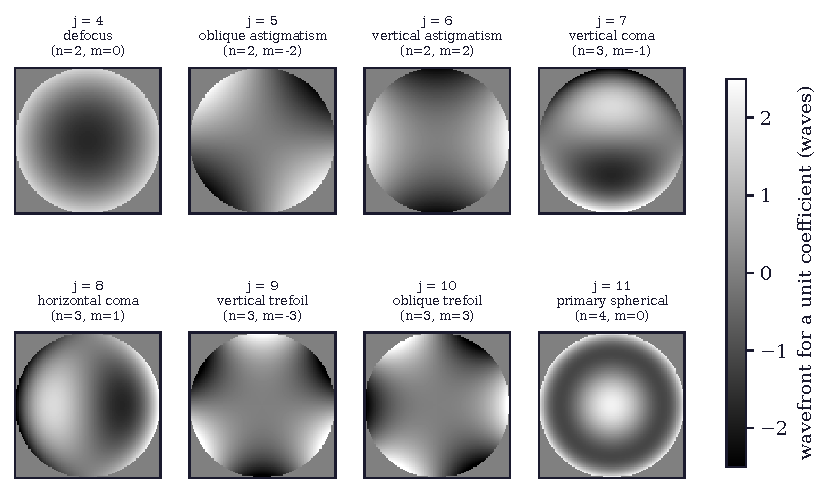
\includegraphics[width=0.9\textwidth]{fig-modes.pdf}
\caption{The eight aberration modes of the design (Noll 4 to 11) on the disc inscribed in the SLM, each for a unit coefficient of one wave, from the basis of the engine; the corners outside the disc are zero. Lighter and darker regions are phase advance and delay, in waves.}
\label{fig:modes}
\end{figure}

\subsection{Metrics and the quantity to be controlled}

Three quantities describe a hologram under a given aberration. The efficiency is the fraction of the input power in the traps, the spread is the relative standard deviation of the weighted intensities across the traps, and the cost compares the intensities with a target level:
\begin{equation}
e=\sum_mI_m,\qquad \sigma=100\,\frac{\operatorname{std}_m\!\big(I_m/w_m\big)}{\operatorname{mean}_m\!\big(I_m/w_m\big)},\qquad L(\phi,a)=\frac{\sum_m\big(I_m(\phi,a)-T_m\big)^2}{\sum_mT_m^2},\quad T_m=\ell\,e_0\,\frac{w_m}{\sum_nw_n},\label{eq:metrics}
\end{equation}
with $\sigma$ in percent, $e_0$ the efficiency of the starting hologram and $\ell$ the target level, a fraction of $e_0$. The spread $\sigma(\phi,a)$ is a random variable when $a$ is random, and what an experimenter fears is its upper tail: a draw of the residual aberration for which the array is uneven.
We therefore score a hologram by the 95th percentile $Q_{95}$ of $\sigma$ over an ensemble of draws of $a$, and by the mean efficiency over the same ensemble, and we compare two holograms by the ratio
\begin{equation}
\rho=\frac{Q_{95}\big[\sigma(\phi_{\mathrm{nom}},a)\big]}{Q_{95}\big[\sigma(\phi,a)\big]},\qquad \eta=\frac{\bar e(\phi)}{\bar e(\phi_{\mathrm{nom}})},\label{eq:ratios}
\end{equation}
where $\phi_{\mathrm{nom}}$ is the hologram of the published method that serves as baseline. A value $\rho>1$ means a lower tail of the spread, $\eta<1$ means a loss of efficiency, and the product tests the pair against $\rho\ge1.25$ and $\eta\ge0.9$ (Section~\ref{sec:design}).

\subsection{The design problem and its assumptions}

The design problem is to find the phase $\phi$ that minimizes the expected cost over the prior of the residual aberration,
\begin{equation}
\min_{\phi\in[0,2\pi)^{N\times N}}\ J(\phi)=\mathbb E_{a\sim\mathcal N(0,s^2I_8)}\,L\big(\phi,a\big),\label{eq:problem}
\end{equation}
and then to evaluate $\rho$ and $\eta$ on draws of $a$ that the optimizer did not use. The assumptions are listed because each bounds the result. (i) The scalar Fourier model of Eq.~\eqref{eq:forward} holds: the traps are on the ideal point-trap model, with no device model (no
pixel crosstalk, no phase quantization, no fill factor) in the forward map. (ii) The aberration is a phase offset on the SLM plane, as in the total-phase sum of the sources; the amplitude of the beam does not change. (iii) The coefficients are independent and Gaussian with one common scale. (iv) The ensemble that evaluates the hologram is drawn
from the same prior as the one that designs it, with a different seed and a different realization of the draws; robustness to other distributions is measured in Section~\ref{sec:results} and is not assumed. (v) The target level and the weights are known and fixed, and the traps are where they are meant to be.

\subsection{Notation}

Table~\ref{tab:notation} collects the symbols of the paper. Every symbol is defined where it first appears in the text, and the table fixes the unit of each one. Hologram phases and aberration phases are in radians, the Zernike coefficients in waves (one wave is $2\pi$ radians of phase), distances in the focal plane in focal bins, that is in units of $\lambda f/(\mathrm{pad}\,N\,p)$, the spacing of the samples of the zero-padded Fourier transform of the SLM field, and intensities as fractions of the power of the input beam, so that the efficiency is a fraction and the spreads are percentages. Indices $j$ run over the SLM pixels, $m$ over the traps and $k$ over the designed modes. The symbols $L$ and $J$ always refer to the cost of Eq.~\eqref{eq:metrics} and its expectation, and $\sigma$ is always the spread of the trap intensities of one realization and not a standard deviation of a prior.

\begin{table}[t]
\centering\small
\caption{Notation of the paper: each symbol with its meaning and its unit; the defaults of the product are the values of the design in Table~\ref{tab:params}.}
\label{tab:notation}
\begin{tabular}{@{}p{2.2cm} p{9.4cm} p{2.6cm}@{}}
\toprule
Symbol & Meaning & Unit\\
\midrule
$N$, $p$ & SLM side in pixels, pixel pitch & 1, \si{\micro\metre}\\
$\phi_j$, $A_j$ & hologram phase and input amplitude of pixel $j$ ($\sum_jA_j^2=N^2$) & rad, 1\\
$\lambda$, $f$ & wavelength, focal length of the lens & \si{\nano\metre}, \si{\milli\metre}\\
$M$, $w_m$ & number of traps, weight of trap $m$ & 1, 1\\
$V_m$, $I_m$ & amplitude and intensity of trap $m$ as a fraction of the input power & 1\\
$Z_k$, $a_k$ & Zernike mode of Noll index $k$ (unit rms over the disc), its coefficient & 1, waves\\
$\psi_j(a)$ & aberration phase on pixel $j$ & rad\\
$s$ & standard deviation of each coefficient in the prior (design amplitude) & waves\\
$\mathcal K$, $K$ & set of designed modes (Noll 4 to 11), their number & 1\\
$e$, $e_0$, $\ell$ & efficiency, efficiency of the start, target level fraction & 1\\
$T_m$ & target intensity of trap $m$, Eq.~\eqref{eq:metrics} & 1\\
$L$, $J$ & cost at one aberration, expected cost & 1\\
$\sigma$, $Q_{95}$ & relative standard deviation of the weighted intensities, its 95th percentile over draws & percent\\
$\rho$, $\eta$ & ratio of the 95th percentiles, ratio of the mean efficiencies, Eq.~\eqref{eq:ratios} & 1\\
$G_{mk}$ & derivative of $I_m$ in the coefficient $a_k$ at the nominal system & 1 per wave\\
$\kappa$ & relative curvature of a trap intensity under displacement & per bin squared\\
\bottomrule
\end{tabular}
\end{table}

\section{Proposed method: the expected-cost hologram}\label{sec:proposed-method}

\subsection{Idea}

A hologram computed for the nominal system places each trap at an optimum of the nominal cost. The aberration then moves the traps off that optimum in directions the nominal cost does not see, and the intensities of the traps change by amounts that depend on how the hologram
phases are arranged, not only on how large the aberration is. Two holograms with the same nominal intensities can respond to the same wavefront error very differently, because the first-order response of each trap intensity to each aberration coefficient is a
property of the phase pattern. The idea is to choose, among the many holograms that equalize the traps at the nominal system, the one whose response to the aberrations of the prior is small, by minimizing the expected cost in Eq.~\eqref{eq:problem} instead of the cost at one point.
The method needs no wavefront measurement and no change of the optical train: it leaves the correction in place and designs for the residual. It starts from the hologram of phase-fixed WGS, which is already a minimizer of the nominal cost to a good approximation, so that the
expected-cost steps trade a small nominal spread and a small efficiency for a flatter response.

\subsection{Derivation}

\paragraph{Step 1, the expected cost.} Because the aberration is an additive phase, the cost at one aberration is the nominal cost at a shifted phase, $L(\phi,a)=L_0(\phi+\psi(a))$, where $L_0$ is the cost of Eq.~\eqref{eq:metrics} at no aberration. The expected cost is
$J(\phi)=\mathbb E_aL_0(\phi+\psi(a))$. Its value and gradient need the nominal cost and gradient at shifted phases only.

\paragraph{Step 2, what the expectation adds to the nominal cost.} For a small prior scale $s$, expand $L_0(\phi+\psi(a))$ to the second order in $a$ and take the expectation, with $\mathbb E a_k=0$ and $\mathbb E a_ka_l=s^2\delta_{kl}$:
\begin{equation}
J(\phi)=L_0(\phi)+\frac{s^2}{2}\sum_{k\in\mathcal K}\frac{\partial^2L_0(\phi+\psi(a))}{\partial a_k^2}\Big|_{a=0}+O(s^4).\label{eq:taylor}
\end{equation}
The second term is the curvature of the cost along each aberration mode. The chain rule, with $\partial\psi_j/\partial a_k=2\pi Z_k(x_j,y_j)$, gives $\partial^2L_0/\partial a_k^2=(2\pi)^2\,\mathbf z_k^{\!\top}\mathbf H(\phi)\,\mathbf z_k$ where $\mathbf z_k$ is the vector of the mode over the pixels and
$\mathbf H$ is the Hessian of $L_0$ in the pixel phases. A hologram with a small penalty sits where the cost is flat along the subspace spanned by the aberration modes.

\paragraph{Step 3, the structure of the curvature.} Write $G_{mk}=\partial I_m/\partial a_k$ for the first-order response of trap $m$ to mode $k$ at the nominal system. By the chain rule with $\partial\psi_j/\partial a_k=2\pi Z_k(x_j,y_j)$ and the derivative of $I_m$ in the pixel phase (Step 5), the response has the closed form
\begin{equation}
G_{mk}=-\frac{4\pi}{N^2}\sum_jA_jZ_k(x_j,y_j)\operatorname{Im}\Big[\bar V_m\,e^{i(\phi_j-\Delta_j^m)}\Big],\label{eq:response}
\end{equation}
a weighted sum over the pixels in which the mode enters as a weight and the phase of the hologram decides the sign: the same mode raises the intensity of one trap and lowers that of another according to the phases the hologram gives the pixels. Differentiating the cost of Eq.~\eqref{eq:metrics} twice gives
\begin{equation}
\frac{\partial^2L_0}{\partial a_k^2}=\frac{2}{\sum_nT_n^2}\Big[\sum_mG_{mk}^2+\sum_m(I_m-T_m)\frac{\partial^2I_m}{\partial a_k^2}\Big],\label{eq:gaussnewton}
\end{equation}
the sum of a Gauss--Newton term, which is non-negative and measures how strongly the intensities respond to the mode, and a residual term, which vanishes when the traps sit at their targets. The robust cost therefore contains the quantity $\sum_{m,k}G_{mk}^2$, the total
first-order intensity variance that the aberration prior induces (Section~\ref{sec:theory} shows that it bounds the expected squared spread).

\paragraph{Step 4, replacing the expectation.} A Monte Carlo average of $L_0$ over random draws of $a$ makes the cost noisy: two evaluations at the same $\phi$ differ, and a line search that needs a decrease between two points cannot decide. A deterministic set removes that noise. The $2K$
sigma points, a pair $\pm s\sqrt K$ on one mode at a time, have mean zero and covariance exactly $s^2I_K$:
\begin{equation}
\mathcal S=\big\{\pm s\sqrt K\,\mathbf e_k\ :\ k\in\mathcal K\big\},\qquad J_{\mathcal S}(\phi)=\frac1{2K}\sum_{\mathbf c\in\mathcal S}L_0\big(\phi+\psi(\mathbf c)\big).\label{eq:sigma}
\end{equation}
For $K=8$ and $s=\parAb$ waves the 16 points lie at $\pm\parAbSqrt$ waves on one mode, a point whose rms wavefront ($\parAbRms$ waves) equals that of the typical draw. Section~\ref{sec:theory} shows that $J_{\mathcal S}$ equals the Gaussian expectation through the second order in $s$. Figure~\ref{fig:design} places the points among the draws of the evaluation ensemble in the plane of two modes, and shows that the sixteen points share one rms wavefront, close to that of the typical draw.

\begin{figure}[t]
\centering
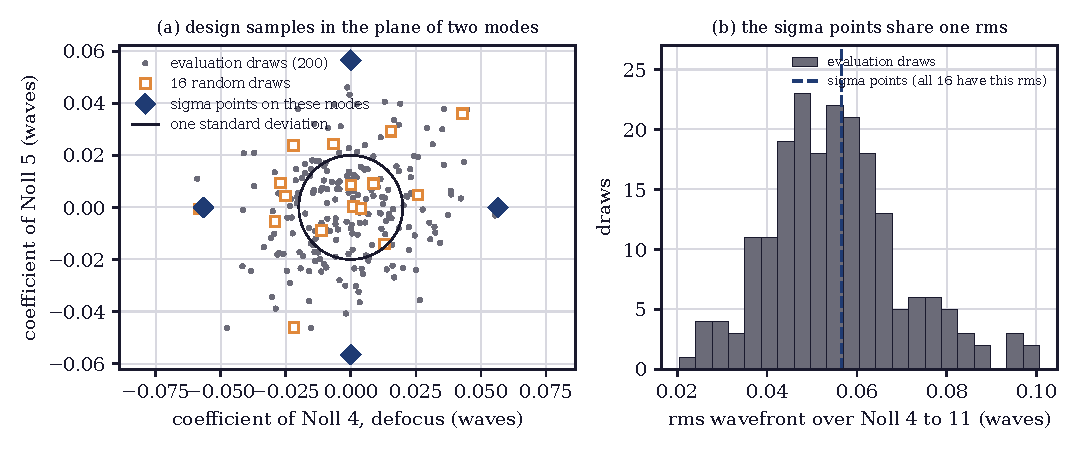
\includegraphics[width=\textwidth]{fig-design.pdf}
\caption{(a) Design samples in the plane of the coefficients of Noll modes 4 and 5: the four sigma points on these two modes, 16 random draws of the alternative design, and the 200 draws of the evaluation ensemble, with the circle of one standard deviation. (b) The rms wavefront over the eight modes of the 200 evaluation draws, and the common rms of the sigma points.}
\label{fig:design}
\end{figure}

\paragraph{Step 5, closed-form gradient.} From Eq.~\eqref{eq:forward}, $\partial I_m/\partial\phi_j=-\frac{2A_j}{N^2}\operatorname{Im}\big[\bar V_me^{i(\phi_j-\Delta_j^m)}\big]$, so for the nominal cost at a shifted phase $\phi'=\phi+\psi(\mathbf c)$,
\begin{equation}
\frac{\partial L_0}{\partial\phi_j}\Big|_{\phi'}=-\frac{4A_j}{N^2\sum_nT_n^2}\operatorname{Im}\Big[\sum_m\big(I_m(\phi')-T_m\big)\,\bar V_m(\phi')\,e^{i(\phi'_j-\Delta_j^m)}\Big],\qquad \nabla_\phi J_{\mathcal S}=\frac1{2K}\sum_{\mathbf c\in\mathcal S}\nabla_\phi L_0\big|_{\phi+\psi(\mathbf c)}.\label{eq:gradient}
\end{equation}
Since the aberration is a constant offset in the phase, the gradient of the expected cost with respect to the pixel phases is the average of the unperturbed gradients at the shifted phases, and each term is one forward and one adjoint evaluation of the point-trap model.

\paragraph{Step 6, the level and the solver.} The target of Eq.~\eqref{eq:metrics} is an absolute level: $T_m=\ell e_0w_m/\sum_nw_n$ with $e_0$ the efficiency of the starting hologram and $\ell=\parLevel$. The scale of the intensities is not refitted during the descent, so that the optimizer cannot lower the
expected cost by dimming all traps. A level below the efficiency of the start asks the hologram to give up a part of its nominal intensity; Section~\ref{sec:ablation} measures the trade-off in $\ell$, and Section~\ref{sec:results} shows that the level plays the role of the mean intensity that the aberrations remove. The cost $J_{\mathcal S}$ is smooth and deterministic, which is what the nonlinear conjugate gradient of Fletcher and
Reeves~\cite{fletcher1964} needs: with the gradient $\mathbf g_i$ at iterate $\phi_i$,
\begin{equation}
\mathbf d_i=-\mathbf g_i+\gamma_i\mathbf d_{i-1},\qquad \gamma_i=\frac{\|\mathbf g_i\|^2}{\|\mathbf g_{i-1}\|^2},\qquad \phi_{i+1}=\phi_i+\alpha_i\mathbf d_i,\label{eq:cg}
\end{equation}
with $\alpha_i$ from a strong-Wolfe line search (constants $c_1=10^{-4}$, $c_2=0.1$; $c_2<1/2$ keeps the directions descent directions)~\cite{nocedal2006}, and a restart from steepest descent when a direction fails.

\paragraph{Variant with random draws.} When the prior includes random displacements of the traps, the cost cannot be written as a function of the phase offset alone, and the product uses $Q$ random draws resampled at every step with Adam~\cite{kingma2015}:
\begin{equation}
\mathbf m_i=\beta_1\mathbf m_{i-1}+(1-\beta_1)\mathbf g_i,\quad \mathbf v_i=\beta_2\mathbf v_{i-1}+(1-\beta_2)\mathbf g_i^2,\quad \phi_{i+1}=\phi_i-\mathrm{lr}\,\frac{\mathbf m_i/(1-\beta_1^i)}{\sqrt{\mathbf v_i/(1-\beta_2^i)}+\epsilon}.\label{eq:adam}
\end{equation}
This design is automatic when a pointing prior is set; it is the design measured in Section~\ref{sec:results} for pointing errors.

\subsection{Design choices}

Four choices shape the method, and each has an alternative that the experiments or the theory discard or leave open. The start is the hologram of phase-fixed WGS and not a random phase or the output of a nominal conjugate-gradient run: the start is already a good minimizer of the nominal cost, it is the baseline of the comparison, and so the expected-cost steps are the only difference between the baseline and the result. A random start would
conflate the benefit of the expected cost with the benefit of reaching a good nominal hologram at all, which some of the published methods of Table~\ref{tab:pub} do not reach at the budgets of the comparison.

The expectation is taken by sigma points and not by random draws because the line search of the solver compares the cost at two points along a direction, and a cost that changes between evaluations at the same point gives no reliable decrease. Random draws held fixed during the descent remove the noise but then optimize for those draws only, and resampled draws need a stochastic optimizer with its smaller steps; the measurements of the ablation put the sigma points ahead of fixed random draws of the same number and of twice the number.

The target level $\ell$ is an absolute intensity that is not rescaled during the descent. If the scale were refitted at each evaluation (the least-squares scale of the cost of Polin et al.~\cite{polin2005}, which the engine offers), the optimizer could lower the expected cost by dimming the traps uniformly; fixing the level at a fraction of the start efficiency prevents it, and gives the user the dial between efficiency and robustness that Section~\ref{sec:ablation} measures. The cost is the sum of squared intensity errors; the same code accepts any even power, and the square is the one that the closed forms of Section~\ref{sec:theory} use.

The designed modes are Noll 4 to 11 and not a larger set because piston changes no intensity and the two tilts move the whole pattern (they belong to the alignment, not to the residual), because Noll 4 to 11 are the modes that the sensorless correction of the product searches and that its acceptance set injects, and because the number of sigma points grows with the number of modes: $2K$ evaluations per cost. A larger set would add points, not change the algorithm, and the ablation shows that a design that does not cover the modes of the ensemble does not protect against them.

\subsection{Algorithm}

Algorithm~\ref{alg:robust} is the aberration design measured in the main experiment, and Algorithm~\ref{alg:sample} the variant with random draws and Adam. The first calls the phase-fixed WGS routine of the product with its documented parameters ($n_{\mathrm{fix}}=12$ weighted iterations before the focal phases are frozen) and then
takes conjugate-gradient steps on the sigma-point cost. Both algorithms return the phase wrapped to $[0,2\pi)$. The descent itself runs on the unwrapped phase, since the field depends on the phase through its exponential and the gradient is a smooth function of it; the wrap at the end changes no intensity. In Algorithm~\ref{alg:robust} the aberration phases of the sixteen points are computed once, because they do not depend on the hologram, so the inner loop is only the forward and adjoint evaluations of the point-trap model. In Algorithm~\ref{alg:sample} the draws change at every step, the traps move with the displacement draw, and the cost is therefore evaluated on a different system at each of the $Q$ draws; its value is a noisy estimate of the expected cost, which is why the algorithm uses a stochastic optimizer and no line search.

\begin{algorithm}[t]
\caption{Aberration-robust hologram with the sigma-point design (the design of the main experiment).}
\label{alg:robust}
\begin{algorithmic}[1]
\Require traps $\{(x_m,y_m,w_m)\}$, prior scale $s$, designed modes $\mathcal K$, level $\ell$, WGS iterations $n_0$, CG iterations $n$, seed
\State $\phi_0\gets$ phase-fixed WGS for $n_0$ iterations from the random-superposition start of the seed
\State $e_0\gets\sum_m|V_m(\phi_0)|^2$; $\ T_m\gets\ell e_0w_m/\sum_nw_n$
\State $\mathcal S\gets\{\pm s\sqrt{|\mathcal K|}\,\mathbf e_k:k\in\mathcal K\}$; precompute $\psi(\mathbf c)$ for every $\mathbf c\in\mathcal S$
\For{$i=1,\dots,n$}
\State $J\gets0$; $\ \mathbf g\gets\mathbf 0$
\For{each $\mathbf c\in\mathcal S$}
\State evaluate $V_m$ at $\phi_{i-1}+\psi(\mathbf c)$ (forward); $L_0$ from Eq.~\eqref{eq:metrics}; $\nabla L_0$ from Eq.~\eqref{eq:gradient} (adjoint)
\State $J\gets J+L_0/|\mathcal S|$; $\ \mathbf g\gets\mathbf g+\nabla L_0/|\mathcal S|$
\EndFor
\State $\mathbf d\gets-\mathbf g+\gamma\mathbf d_{\mathrm{prev}}$ (Eq.~\eqref{eq:cg}); restart with $\mathbf d\gets-\mathbf g$ if $\mathbf g^{\top}\mathbf d\ge0$
\State find $\alpha$ by the strong-Wolfe search (each trial repeats the inner loop); $\ \phi_i\gets\phi_{i-1}+\alpha\mathbf d$
\EndFor
\State \Return $\phi_n\bmod2\pi$
\end{algorithmic}
\end{algorithm}

\begin{algorithm}[t]
\caption{Variant with random draws, Adam and a pointing prior.}
\label{alg:sample}
\begin{algorithmic}[1]
\Require as Algorithm~\ref{alg:robust}, plus the pointing scale $s_p$ in focal bins, draws per step $Q$, rate $\mathrm{lr}$
\State $\phi_0$, $e_0$, $T_m$ as in Algorithm~\ref{alg:robust}; $\mathbf m,\mathbf v\gets\mathbf 0$
\For{$i=1,\dots,n$}
\For{$q=1,\dots,Q$}
\State draw $a\sim\mathcal N(0,s^2I_K)$ and displacements $d^x_m,d^y_m\sim\mathcal N(0,s_p^2)$ bins for every trap
\State evaluate $L_0$ and $\nabla L_0$ at $\phi_{i-1}+\psi(a)$ for the traps moved by $(d^x_m,d^y_m)$; average over $q$
\EndFor
\State update $\mathbf m,\mathbf v$ and $\phi_i$ by Eq.~\eqref{eq:adam}
\EndFor
\State \Return $\phi_n\bmod2\pi$
\end{algorithmic}
\end{algorithm}

\subsection{Parameters}

Table~\ref{tab:params} lists every parameter with its value in the experiments and where the value comes from. The values are those of the implementation; the design amplitude $s$ is a choice of the product that the paper states and measures (Sections~\ref{sec:ablation} and~\ref{sec:results}), not a figure
taken from a published instrument, and the number of random draws per step ($Q=\parQ$) follows the range of 8 to 32 samples per iteration recorded in the research that preceded the implementation. Two of the parameters carry most of the behaviour and are therefore varied in the ablation: the design amplitude $s$, which sets how far the sigma points sit from the nominal system, and the level $\ell$, which sets how much room the hologram has to move without paying nominal error. The others are conventions of the solver (the Wolfe constants are the textbook ones and the Adam constants are those of its authors) or of the start (the 30 iterations of phase-fixed WGS are the iteration count at which the baseline of the comparison is scored).

\begin{table}[t]
\centering\small
\caption{Parameters of the aberration-robust hologram: the value used in the experiments and its origin. The values are read from the implementation by the measurement script.}
\label{tab:params}
\begin{tabular}{@{}p{3.1cm} p{2.4cm} p{8.6cm}@{}}
\toprule
Parameter & Value & Origin\\
\midrule
Design amplitude $s$ & \parAb{} waves per mode & stated choice of the product; ensemble rms \parAbRms{} waves, Strehl about 0.88\\
Designed modes $\mathcal K$ & Noll 4 to 11 & defocus, astigmatisms, comas, trefoils and spherical; piston and tilts excluded\\
Sigma points & 16 & $\pm s\sqrt8$ on one mode at a time\\
Target level $\ell$ & \parLevel & trade-off measured in Section~\ref{sec:ablation}\\
Start & phase-fixed WGS, \parWarm{} iterations & the baseline method, with $n_{\mathrm{fix}}=12$ weighted iterations before the phase is frozen\\
CG iterations $n$ & \parIters{} & budget of the acceptance test\\
Line search & strong Wolfe & $c_1=10^{-4}$, $c_2=0.1$, cubic interpolation; first trial moves the largest pixel by 0.1 rad\\
Draws per step $Q$ & \parQ{} & range of 8 to 32 per iteration of the research record\\
Adam rate & \parLr{} & $\beta_1=0.9$, $\beta_2=0.999$, $\epsilon=10^{-8}$\\
\bottomrule
\end{tabular}
\end{table}

\subsection{Complexity}

One evaluation of the cost and gradient at one sigma point costs a forward and an adjoint evaluation of the point-trap model, each a product of $N\times N$ and $N\times M$ matrices in the separable form, $O(N^2M)$ operations. One conjugate-gradient iteration evaluates the $2K=16$ sigma points once per trial step of
the line search, so the cost of a run is $O\big(n\,t_{\mathrm{ls}}\,2K\,N^2M\big)$ with $t_{\mathrm{ls}}$ the number of trial steps per iteration, against $O(n\,t_{\mathrm{ls}}N^2M)$ for conjugate gradient on the nominal cost, a factor $2K$ more. The ensemble evaluation of the result is $200$ forward evaluations per hologram.
In the experiments ($N=256$, $M=100$, $n=\parIters$) one run of the robust hologram took a median of \runSeconds{} seconds of wall-clock time per seed with \workersUsed{} processes sharing the machine, so the figure is an upper bound of an unloaded run. The cost of a run is linear in the number of sigma points, and so in the number of designed modes. The method is a design computed once per array, offline,
and is not a method for the live loop of a rearrangement.

\subsection{Implementation}

The method is implemented in the repository of the product as the module \texttt{pipeline.model.holo.methods.beyond.b4\_robust}, which exposes the run function with the parameters of Table~\ref{tab:params}, the sigma-point generator and an ensemble evaluator that returns the efficiency, the 95th percentile and the sorted spreads
over a seeded ensemble. It builds on the cost class and the conjugate-gradient and Adam routines of the shared optimization module and on the phase-fixed WGS of the weighted-GS family, so that its start is the published method itself and not a copy of its equations. All randomness comes from a portable
generator (xoshiro128** seeded by SplitMix32) so that a seed gives the same hologram on every machine. The experiments of this paper call the module through its public functions and, for the ablation, a replica of the sigma-point loop that takes the design samples as an argument; the replica reproduces the module's hologram on the default
configuration to \replicaDiff{} rad in the largest pixel phase.

\section{Theory: why the expected cost should lower the spread}\label{sec:theory}

\subsection{Setting and standing conditions}

Let $f(a)=L_0(\phi+\psi(a))$ for a fixed hologram $\phi$. Because $\psi_j(a)$ is linear in $a$ and the forward map of Eq.~\eqref{eq:forward} is a finite sum of complex exponentials, $f$ is a real-analytic function of $a\in\mathbb R^K$, so every derivative exists and the Taylor series
of $f$ at the origin has an infinite radius of convergence. The statements below are expansions in the prior scale $s$ with the hologram fixed, and they hold under three conditions that the experiments check and do not assume. (C1) The aberration phase is small enough for
a low-order expansion of the field to describe the intensity: the Strehl ratio of the ensemble is near one, which for the design prior is about $0.88$, so that a first-order model of the traps has an error of the order of the squared phase offset. (C2) The coefficients are independent, centred and Gaussian with the common scale $s$, the assumption
of Eq.~\eqref{eq:problem}. (C3) The traps have equal weights, so that the weighted intensity of Eq.~\eqref{eq:metrics} is the intensity itself; unequal weights change the constants and not the statements. The first two propositions concern the cost that the optimizer sees, the third the spread that the experimenter
sees, and the fourth the first-order and second-order structure of the spread under displacements of the traps.

\subsection{Proposition 1: the sigma points match the expectation to second order}

\paragraph{Statement.} For any real-analytic $f$ on $\mathbb R^K$, the average of $f$ over the $2K$ sigma points of Eq.~\eqref{eq:sigma} and the expectation of $f(a)$ for $a\sim\mathcal N(0,s^2I_K)$ agree through the second order in $s$,
\begin{equation}
\frac1{2K}\sum_{\mathbf c\in\mathcal S}f(\mathbf c)-\mathbb E f(a)=\frac{s^4}8\Big[\frac K3\sum_k\partial_k^4f(0)-\sum_{k,l}\partial_k^2\partial_l^2f(0)\Big]+O(s^6),\label{eq:sigmaerror}
\end{equation}
and both equal $f(0)+\frac{s^2}2\sum_k\partial_k^2f(0)$ up to that error.

\paragraph{Proof.} Expand $f(\mathbf c)=\sum_{r\ge0}\frac1{r!}(\mathbf c\!\cdot\!\nabla)^rf(0)$. A sigma point $\pm c\,\mathbf e_k$ with $c=s\sqrt K$ contributes $\sum_r\frac{(\pm c)^r}{r!}\partial_k^rf(0)$; the pair averages to $\sum_{r\text{ even}}\frac{c^r}{r!}\partial_k^rf(0)$ because the odd terms cancel. Averaging over the $K$ modes with equal weight gives
$f(0)+\frac{c^2}{2K}\sum_k\partial_k^2f(0)+\frac{c^4}{24K}\sum_k\partial_k^4f(0)+O(c^6)$, and $c^2/K=s^2$, $c^4/K=Ks^4$. For the Gaussian, odd moments vanish and the moments of a centred Gaussian vector are $\mathbb E[a_ia_j]=s^2\delta_{ij}$ and $\mathbb E[a_ia_ja_ka_l]=s^4(\delta_{ij}\delta_{kl}+\delta_{ik}\delta_{jl}+\delta_{il}\delta_{jk})$, so
$\mathbb Ef(a)=f(0)+\frac{s^2}2\sum_k\partial_k^2f(0)+\frac{s^4}8\sum_{k,l}\partial_k^2\partial_l^2f(0)+O(s^6)$. Subtracting the two series gives Eq.~\eqref{eq:sigmaerror}. \hfill$\square$

\paragraph{Reading.} The sigma points are exact for the mean and the covariance and are blind to the mixed fourth derivatives; they weight the pure fourth derivatives by $K/3$, which is $8/3$ for the eight modes against the factor one of the Gaussian. The error is of the order of $s^4$ times fourth derivatives of the cost. The
sigma-point cost is therefore a faithful stand-in for the expectation as long as the second-order terms dominate, which is condition (C1), and it is not a quadrature for tails of the prior: the points sit at a fixed distance $s\sqrt K$ from the origin, which is the typical radius of a draw of $K$ coefficients, and not at the rare large draws that set the upper tail of the spread.

\subsection{Proposition 2: the robust cost is the nominal cost plus a curvature along the aberration modes}

\paragraph{Statement.} Let $G_{mk}=\partial I_m/\partial a_k$ at $a=0$ and $T_{\Sigma}=\sum_nT_n^2$. Then
\begin{equation}
J_{\mathcal S}(\phi)=L_0(\phi)+\frac{s^2}{T_\Sigma}\Big[\sum_{m,k}G_{mk}^2+\sum_m(I_m-T_m)\sum_k\frac{\partial^2I_m}{\partial a_k^2}\Big]+O(s^4),\label{eq:curvature}
\end{equation}
where all quantities are evaluated at the nominal system. The first bracketed term is non-negative, and it is the only term that survives when the traps sit at their targets.

\paragraph{Proof.} Apply Proposition 1 to $f=L_0(\phi+\psi(\cdot))$ to replace $J_{\mathcal S}$ by $L_0+\frac{s^2}2\sum_k\partial_k^2f(0)+O(s^4)$, and use Eq.~\eqref{eq:gaussnewton}, which follows from $L_0=T_\Sigma^{-1}\sum_m(I_m-T_m)^2$ by the product rule: $\partial_k^2L_0=\frac2{T_\Sigma}\sum_m\big[(\partial_kI_m)^2+(I_m-T_m)\partial_k^2I_m\big]$. Multiplying by $s^2/2$ gives Eq.~\eqref{eq:curvature}. \hfill$\square$

\paragraph{Reading.} Minimizing $J_{\mathcal S}$ over $\phi$ lowers the first-order intensity variance $s^2\sum_{m,k}G_{mk}^2$ that the aberration prior induces, at the price of the nominal cost $L_0$. The nominal cost at the start is not zero, because the target level of Eq.~\eqref{eq:metrics} is a fraction $\ell$ of the efficiency of the start, so both bracketed terms of Eq.~\eqref{eq:curvature} matter and Section~\ref{sec:results} reports them separately. A hologram whose traps
respond weakly to the eight modes is preferred; this is a property of the phase pattern among the many that equalize the traps, which is why the choice matters at all.

\subsection{Proposition 3: the first-order spread and its bound by the penalty}

\paragraph{Statement.} Let $\sigma_0$ be the spread at the nominal system, $\bar I$ the mean nominal intensity, $\mathbf G_c$ the matrix $G$ with the mean over traps subtracted from each column, and $\Gamma=\dfrac{100^2}{M\bar I^2}\,\mathbf G_c^{\top}\mathbf G_c$. To first order in $a$,
\begin{equation}
\sigma(a)^2\approx\sigma_0^2+2\,\mathbf b^{\top}a+a^{\top}\Gamma a,\qquad \mathbb E\,\sigma^2\approx\sigma_0^2+s^2\operatorname{tr}\Gamma\ \le\ \sigma_0^2+\frac{100^2s^2}{M\bar I^2}\sum_{m,k}G_{mk}^2=\sigma_0^2+100^2\,\frac{T_m^2}{\bar I^2}\,\frac{s^2\sum_{m,k}G_{mk}^2}{T_\Sigma},\label{eq:spreadbound}
\end{equation}
with $\mathbf b=\frac{100^2}{M\bar I^2}\mathbf G_c^{\top}(I-\bar I)$ a vector that vanishes when the nominal intensities are equal and, for equal weights, $T_m^2=T_\Sigma/M$. When the nominal spread is zero, $\sigma(a)^2=a^{\top}\Gamma a$ is a positive semidefinite quadratic form in a Gaussian vector, that is a weighted sum $s^2\sum_i\lambda_i\xi_i^2$ of independent unit chi-square variables with the eigenvalues $\lambda_i$ of $\Gamma$, and the 95th percentile of $\sigma$
is the square root of the 95th percentile of that sum.

\paragraph{Proof.} Write $I_m(a)\approx I_m+\sum_kG_{mk}a_k$; the mean over traps is $\bar I+\bar{\mathbf G}\!\cdot\!a$ and the centred intensity is $(I_m-\bar I)+(\mathbf G_c a)_m$. The squared spread is $100^2$ times the mean over traps of the squared centred intensity over the squared mean intensity; to first order in $a$ the denominator is $\bar I^2$ times a factor $1+O(a)$ that multiplies terms already of first or second order.
Expanding the square gives a constant (the nominal variance $\sigma_0^2\bar I^2/100^2$), a term linear in $a$ proportional to $\sum_m(I_m-\bar I)(\mathbf G_ca)_m$, which is zero when the nominal intensities are equal, and the quadratic form $\frac1M\|\mathbf G_ca\|^2$. The expectation of $a^{\top}\Gamma a$ is $s^2\operatorname{tr}\Gamma$ by $\mathbb E[aa^{\top}]=s^2I$, and
$\operatorname{tr}\Gamma\le\frac{100^2}{M\bar I^2}\|\mathbf G\|_F^2$ because subtracting the column means removes a non-negative amount of squared norm. The last equality in Eq.~\eqref{eq:spreadbound} is a rewriting with $T_\Sigma=MT_m^2$. The distribution of the quadratic form follows from the eigendecomposition of $\Gamma$ and the rotation invariance of the Gaussian. \hfill$\square$

\paragraph{Reading.} The bound states that the expected squared spread caused by the aberration is at most a constant times the Gauss--Newton part of the robust penalty of Proposition 2, with the constant $100^2T_m^2/\bar I^2$ that is the squared ratio of the target to the achieved mean intensity. The optimizer therefore lowers a quantity that bounds the expected squared spread, and this is the sense in which the expected cost is the right
cost for the metric. It is not a guarantee on the tail: the 95th percentile depends on the whole spectrum of $\Gamma$, and a hologram that lowers the trace can leave a large eigenvalue; the experiment measures the percentile.

\subsection{Proposition 4: displacements of the traps, a slope term and a curvature floor}

\paragraph{Statement.} Let trap $m$ be displaced by $d$ focal bins along $x$, and let $k_j$ be the phase gradient per bin that the displacement adds to pixel $j$, $k_j=2\pi x_j/(\mathrm{pad}\,N\,p)$ with $\mathrm{pad}$ the zero-padding factor of the focal sampling. For a displacement vector $\mathbf d=(d_x,d_y)$ the relative change of the intensity of trap $m$ is
$\varepsilon_m(\mathbf d)=\mathbf s_m\!\cdot\!\mathbf d-\tfrac12\kappa_m|\mathbf d|^2+O(|\mathbf d|^3)$, with the slope $\mathbf s_m=\nabla_{\mathbf d}I_m/I_m$ and the curvature $\kappa_m$. If the phases of the pixels are aligned on trap $m$, that is $\phi_j-\Delta_j^m$ is the same for all $j$ up to a constant, then $\mathbf s_m=0$ and
\begin{equation}
\kappa_m=\kappa_{\mathrm{ap}}=2\operatorname{Var}_A(k)=2\Big[\sum_jw_jk_j^2-\Big(\sum_jw_jk_j\Big)^2\Big],\qquad w_j=\frac{A_j}{\sum_nA_n}.\label{eq:curv}
\end{equation}
For independent isotropic displacements of standard deviation $s_p$ bins in $x$ and $y$, and traps with slopes $\mathbf s_m$ and a common curvature $\kappa$, the relative standard deviation of the trap intensities is, to leading order,
\begin{equation}
\sigma_{\mathrm{point}}\approx100\sqrt{\overline{|\mathbf s|^2}\,s_p^2+\kappa^2s_p^4},\qquad\overline{|\mathbf s|^2}=\frac1M\sum_m|\mathbf s_m|^2.\label{eq:pointing}
\end{equation}
The curvature scales with the second moment of the beam over the SLM, hence with the inverse square of the width of the focused spot; the slope is a property of the hologram.

\paragraph{Proof.} With aligned phases the field is $V(d)\propto\sum_jA_je^{-ik_jd}$, whose derivatives at zero are $V'=-i\sum_jA_jk_j$ and $V''=-\sum_jA_jk_j^2$ (up to the constant). The intensity $I=|V|^2$ has $I''=2\operatorname{Re}(\bar VV'')+2|V'|^2=-2(\sum A)(\sum Ak^2)+2(\sum Ak)^2$, so $-I''/I=2[\langle k^2\rangle-\langle k\rangle^2]$ with the average weighted by $A_j$, and
$I'=0$ because $V'$ is purely imaginary while $V$ is real. For general phases the expansion of $\varepsilon_m$ is the Taylor expansion of $I_m(\mathbf d)/I_m(0)$. With independent displacements, $\varepsilon_m$ has mean $-\kappa s_p^2$ (since $\mathbb E|\mathbf d|^2=2s_p^2$) and variance $|\mathbf s_m|^2s_p^2+\tfrac14\kappa^2\operatorname{Var}(|\mathbf d|^2)=|\mathbf s_m|^2s_p^2+\kappa^2s_p^4$, because
$|\mathbf d|^2=s_p^2\chi_2^2$ has variance $4s_p^4$ and the cross moment of the linear and the quadratic term vanishes by symmetry. Taking the standard deviation over the traps of one realization, with the displacements of the traps independent, gives Eq.~\eqref{eq:pointing}. \hfill$\square$

\paragraph{Reading and status.} The aligned-phase value is exact only for that case. For a real hologram the pixel phases are not aligned on every trap, the slope does not vanish, and the statement that the curvature of an optimized hologram is close to $\kappa_{\mathrm{ap}}$ is a conjecture, which Section~\ref{sec:results} tests by finite differences on the holograms of phase-fixed WGS and of the robust hologram, together with the model of Eq.~\eqref{eq:pointing} against the measured spread.
If both hold, a design can lower the spread under displacement by lowering the slope, and can go no lower than the floor $100\kappa s_p^2$ without changing the spot width; halving $\kappa$ needs a spot $\sqrt2\approx1.4$ times wider, which changes the beam and not the hologram. The expected-cost design for aberrations does not act on the slope, which is a different first-order response from the one it lowers, and the proposition therefore predicts that it gives no gain under displacements and
that a design with a displacement prior can approach the floor but not pass it.

\subsection{Conditions and what the theory leaves open}

The four propositions are statements about a fixed hologram and a small prior. They do not say that the optimizer reaches a global minimum of $J_{\mathcal S}$ (the cost is non-convex in the phases, and the descent starts from phase-fixed WGS and ends where the budget ends); they do not give the improvement as a function of $s$, which depends on the Hessian of the cost at the start;
and they do not bound the nominal spread that the optimizer is allowed to add, which is set by the target level $\ell$ and the iterations. Proposition 2 explains why the nominal cost may rise: the design moves to a point of lower response and higher nominal cost, and the target level decides how far. The conditions (C1) to (C3) are the places where the
theory can fail: a prior far from small (C1), a correlated or non-Gaussian residual (C2), and unequal weights (C3). The ablation and the mismatch experiments of Section~\ref{sec:results} test the first two.

\section{Experimental design}\label{sec:design}

\subsection{Hypotheses}

The experiments test the following hypotheses, each stated with the quantity that confirms or refutes it. Where the statement carries a threshold, the threshold is the acceptance criterion of the product's method record for this method, set before the repeated measurements of this paper.
\begin{description}
\item[H1, aberration spread.] Over the ensemble of \parNens{} aberration draws, the 95th percentile of the spread of the robust hologram is at least $1.25$ times lower than that of phase-fixed WGS ($\rho\ge1.25$), on every seed of the holograms. Refuted by one seed below the threshold.
\item[H2, efficiency.] The mean efficiency over the ensemble is at least $0.9$ of that of phase-fixed WGS ($\eta\ge0.9$).
\item[H3, the expected cost is the cause.] The gain does not come from the extra conjugate-gradient iterations or from a gradient method on the nominal cost: conjugate gradient on the nominal cost (the same solver and budget with a single design point at the origin) and the published gradient methods of the product give $\rho$ below $1.25$ against phase-fixed WGS.
\item[H4, deterministic samples.] For the same number of design samples, the sigma points give a larger $\rho$ than random draws, because the cost has no sampling noise.
\item[H5, first-order theory.] The first-order model of Proposition 3 reproduces the spread of each draw (Pearson correlation of at least $0.9$ between the predicted and the measured spread), and the measured mean squared spread lies below the bound of Eq.~\eqref{eq:spreadbound}.
\item[H6, pointing errors.] The same expected cost with a displacement prior of $0.15$ focal bins reaches $\rho\ge1.25$ on the joint ensemble of aberrations and displacements. The theory of Proposition 4 predicts that it does not.
\item[H7, mismatch.] The gain persists when the evaluation ensemble differs from the design prior: other amplitudes, and modes outside Noll 4 to 11. The theory gives no prediction beyond (C1) and (C2), so this is an exploration, and either outcome is reported.
\end{description}

\subsection{Data and task provenance}

The experiments use no external data. The task is the one of the acceptance test of the method in the repository of the product: a $10\times10$ square lattice of $M=100$ equal traps, eight focal bins apart, on an SLM of $256\times256$ pixels padded by a factor of two, with a wavelength of 850 nm, a focal length of 250 mm, a pixel pitch of
12.5 micrometres and a Gaussian input beam whose $1/e^2$ intensity waist equals half the SLM side. The ensemble is \parNens{} draws of the eight Noll 4 to 11 coefficients from the portable pseudo-random generator of the product (xoshiro128** seeded by SplitMix32, Box--Muller normals), seed \parEnsSeed, with the standard deviation of $\parAb$ waves per mode; the design of the method draws no random numbers
(the sigma points are deterministic) and the start of phase-fixed WGS draws its random phases from the seed of the hologram, so the evaluation ensemble and the design are independent. Ensembles of five other seeds (1001 to 1005) test the holograms on new draws of the same prior. The committed bake of the product, which holds the relative standard deviation of every method on the
cases of the studio over three seeds, supplies the cross-check on cases other than the task (Section~\ref{sec:results}). The task is small by the standards of the arrays of Section~\ref{sec:intro}; it is chosen because phase-fixed WGS reaches a near-zero nominal spread on it, so that the spread under aberration is the quantity under study and not a residual of the nominal design.

\subsection{Published methods run on the same task}

The comparison runs the published methods through the engine of the product, on the same task, seeds and ensemble, and does not rely on reported numbers. The baseline is phase-fixed WGS~\cite{kim2019} (30 iterations, 12 weighted iterations before the phase is frozen), which is also the start of the proposed method, so that the comparison isolates the expected-cost steps.
The other methods are Gerchberg--Saxton, the generalized adaptive additive variant and weighted GS with their weights~\cite{dileonardo2007} (30 iterations each), conjugate gradient on the nominal cost with 40 iterations~\cite{harte2014}, and Wirtinger gradients with Adam, 40 iterations~\cite{chakravarthula2019}. One more control, central to H3, is the sigma-point loop of the proposed method with a single design point
at the origin: the same solver, budget, level and start, and the nominal cost only. Learned generators~\cite{eybposh2020,shi2021} and models of the SLM device~\cite{schroff2023,persson2012} are not compared, because they address other quantities (volumes, crosstalk) and the task of this paper has an ideal device. A global Zernike correction~\cite{nogrette2014} is not a competitor but a
precondition: the ensemble models what remains after it.

\subsection{Metrics}

The metrics are those of Eqs.~\eqref{eq:metrics} and~\eqref{eq:ratios}: the 95th percentile $Q_{95}$ of the spread over the ensemble, the mean spread, the maximum, the mean efficiency, and the ratios $\rho$ and $\eta$. For one hologram, the fraction of draws on which the robust hologram has the lower spread, $W/n$ with $W=\sum_{r=1}^n\mathbf 1[\sigma_r^{\mathrm{rob}}<\sigma_r^{\mathrm{nom}}]$, is tested against the null of equal chances by the exact two-sided binomial sign test,
\begin{equation}
p=\min\Big\{1,\ 2^{1-n}\sum_{i=0}^{\min(W,n-W)}\binom ni\Big\},\label{eq:sign}
\end{equation}
where the draws are paired because both holograms are scored on the same draw. The first-order model of Proposition 3 is scored by the Pearson correlation between the predicted and the measured spread per draw, the ratio of the predicted to the measured 95th percentile, and the comparison of $\sigma_0^2+s^2\operatorname{tr}\Gamma$ with the measured mean squared spread. The pointing curvature of
Proposition 4 is the finite-difference quantity $\kappa=-\big[I(\delta)+I(-\delta)-2I(0)\big]/(\delta^2I(0))$ with $\delta=\parCurvDelta{}$ bin, averaged over the traps, and $\kappa_{\mathrm{ap}}$ is computed from the beam by Eq.~\eqref{eq:curv}. The slope of the trap intensity under displacement, $(I(\delta)-I(-\delta))/(2\delta I(0))$ per bin, is computed the same way and enters the pointing model of Section~\ref{sec:results}.

\subsection{Protocol}

For each seed of the holograms ($1,\dots,\nSeedsAll$) the protocol is the following. The baseline hologram is computed by 30 iterations of phase-fixed WGS from the random start of the seed; the robust hologram is computed by $\parIters$ conjugate-gradient iterations of Algorithm~\ref{alg:robust} from that same hologram; both are scored on the ensemble of seed \parEnsSeed. The ten seeds are the unit of replication for the main comparison; the first three
seeds, which are the seeds of the acceptance test of the method, feed all the other parts (the held-out ensembles, the published methods, the ablation, the theory check, the mismatch and the pointing experiments), because each of those costs a full run of the optimizer per configuration. All methods take their seed through the portable generator, the runs are deterministic and a rerun gives the same numbers up to the floating point of the machine's FFT.
The main measurement ran \workersUsed{} processes in parallel and took \totalMinutes{} minutes; the pointing-only part, run afterwards on the stored holograms with \pointonlyWorkers{} processes, took \pointonlyMinutes{} minutes. The script that runs it is the only source of the numbers, tables and figures of this paper.

\subsection{Planned ablations}

The ablation varies one element of the method at a time on the first three seeds and scores each variant on the same ensemble against the same baseline hologram. The elements are: the kind and number of design samples (the sigma points; $4$, $8$, $16$ and $32$ fixed random draws with the same solver; resampled random draws with Adam; the single point at the origin that serves as control for H3); the modes in the design (Noll 4 only; 4 to 6; 4 to 8; 9 to 11; the full 4 to 11);
the design amplitude ($0.005$ to $0.04$ waves per mode, evaluated on the fixed ensemble of $\parAb$ waves); the target level $\ell$ ($0.80$ to $1.00$); and the number of conjugate-gradient iterations ($5$ to $80$). Each variant is the replica of the sigma-point loop with one argument changed; the replica is verified against the module on the default configuration. The results are in Section~\ref{sec:ablation}. The pointing experiments add two variables of their own: the displacement prior, with and without the aberration prior in the design and in the ensemble, and the budget of the sampled design (20 and 100 Adam steps).

\subsection{Statistics}

Each ratio has an interval. For one seed, the paired bootstrap resamples the ensemble draws with replacement 2000 times and recomputes both 95th percentiles in each resample; the interval is the 2.5th to 97.5th percentile of the resampled ratios, and it measures the uncertainty that comes from the finite ensemble. Across seeds, the median is the summary of the ratio, with its range over three seeds and, over ten seeds, a bootstrap interval of the median from $10^4$ resamples of the seeds.
The seeds of the holograms and the draws of the ensemble are the two sources of variation, and they are reported separately: the first by the range over seeds, the second by the bootstrap per seed. There is no correction for multiple comparisons because the hypotheses are few, fixed in advance, and each is judged on its own threshold, not on a significance level. The ablation reports the median and the range of three seeds, which is a statement about the seed-to-seed
variation of the design and not a test of a difference between variants.

\section{Results}\label{sec:results}

\subsection{Spread under residual aberrations}

Table~\ref{tab:main} gives, for each of the \nSeedsAll{} seeds of the holograms, the 95th percentile of the relative standard deviation over the ensemble of \parNens{} aberration draws for phase-fixed WGS and for the robust hologram, their ratio $\rho$ with the paired bootstrap interval over the draws, the efficiency ratio $\eta$, and the number of draws on which the robust hologram has the lower spread. On the three seeds of the acceptance test the median ratio is
\ratioMed{} (range \ratioMin{} to \ratioMax) at a median efficiency ratio of \effRatioMed{} (\effRatioMin{} to \effRatioMax); over all \nSeedsAll{} seeds the median is \ratioAllMed{} with a bootstrap interval of the median from \ratioAllCiLo{} to \ratioAllCiHi, and the efficiency ratio stays between \effAllMin{} and \effAllMax. Hypothesis H1 holds on \seedsPassing{} of \nSeedsAll{} seeds and H2 on \seedsEffPassing{} of \nSeedsAll.
The bootstrap intervals of single seeds are wide, from about \ratioOneLo{} to \ratioOneHi{} for seed 1, and \ciBelowN{} of the \nSeedsAll{} intervals have a lower end under $1.25$: the criterion is met by every seed's point estimate and by the median over seeds, not by every interval of a single $200$-draw ensemble.

\begin{table}[t]
\centering\small
\caption{Spread under residual aberrations on the $10\times10$ task: 95th percentile of the relative standard deviation (percent) over 200 draws for phase-fixed WGS and for the robust hologram, their ratio with the 95 percent paired bootstrap interval over the draws, the efficiency ratio, and the draws on which the robust hologram has the lower spread, for each seed of the holograms.}
\label{tab:main}
\begin{tabular}{@{}r r r l r r@{}}
\toprule
Seed & $Q_{95}$ WGS & $Q_{95}$ robust & $\rho$ [interval] & $\eta$ & draws won\\
\midrule
1 & 6.192 & 3.947 & 1.57 [1.34, 1.73] & 0.981 & 200/200 \\
2 & 5.983 & 4.220 & 1.42 [1.29, 1.70] & 0.983 & 200/200 \\
3 & 6.068 & 4.230 & 1.43 [1.27, 1.61] & 0.982 & 200/200 \\
4 & 5.925 & 4.050 & 1.46 [1.28, 1.65] & 0.983 & 200/200 \\
5 & 5.923 & 4.376 & 1.35 [1.27, 1.66] & 0.982 & 200/200 \\
6 & 5.955 & 3.906 & 1.52 [1.21, 1.62] & 0.982 & 200/200 \\
7 & 6.080 & 4.151 & 1.46 [1.26, 1.64] & 0.982 & 200/200 \\
8 & 5.965 & 4.362 & 1.37 [1.31, 1.64] & 0.982 & 200/200 \\
9 & 5.948 & 4.312 & 1.38 [1.29, 1.64] & 0.982 & 200/200 \\
10 & 5.856 & 4.056 & 1.44 [1.23, 1.61] & 0.982 & 200/200
\\
\midrule
Median, seeds 1 to 3 & & & \ratioMed{} (\ratioMin{} to \ratioMax) & \effRatioMed & \\
Median, \nSeedsAll{} seeds & & & \ratioAllMed{} [\ratioAllCiLo, \ratioAllCiHi] & \effAllMed & \\
\bottomrule
\end{tabular}
\end{table}

Figure~\ref{fig:ecdf} shows the whole distribution for seed 1. The robust hologram has the lower spread on \winsOne{} of the \parNens{} draws (exact sign test, $p=\signPOne$), its median spread is \evalMedBfour{} percent against \evalMedNom{}, its mean \evalMeanBfour{} against \evalMeanNom, and its largest spread \evalMaxBfour{} against \evalMaxNom{} percent. The whole distribution moves left, so the gain is not confined to the tail that the 95th percentile selects; the ratio of the means is \meanRatioOne{} on this seed, a little larger than the ratio of the 95th percentiles of \ratioOne.
Figure~\ref{fig:seeds} shows the ratio and the efficiency ratio for every seed: the ratios range from \ratioAllMin{} to \ratioAllMax{} and the efficiency ratio is within \effAllMin{} to \effAllMax, a seed-to-seed variation of the design that is small against the gain.

\begin{figure}[t]
\centering
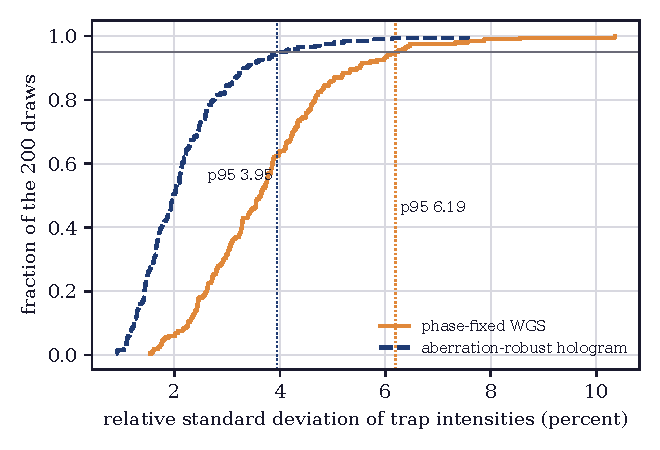
\includegraphics[width=0.62\textwidth]{fig-ecdf.pdf}
\caption{Empirical distribution function over the 200 aberration draws of the relative standard deviation of the 100 trap intensities (percent), for phase-fixed WGS (solid) and the robust hologram (dashed), seed 1. The dotted verticals mark the 95th percentiles, the horizontal line the 95 percent level.}
\label{fig:ecdf}
\end{figure}

\begin{figure}[t]
\centering
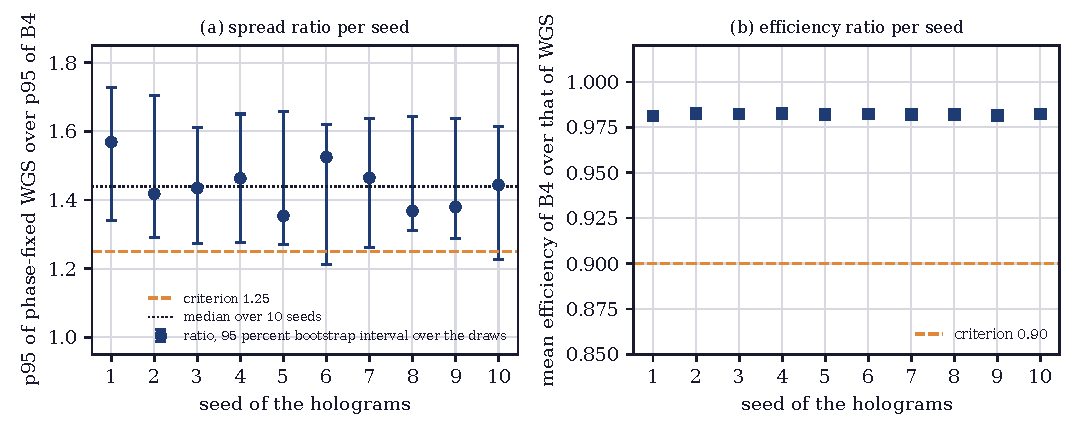
\includegraphics[width=\textwidth]{fig-seeds.pdf}
\caption{(a) Ratio of the 95th percentiles of phase-fixed WGS and of the robust hologram for each of ten seeds of the holograms, with the paired bootstrap interval over the 200 draws, the criterion of 1.25 and the median over seeds. (b) Ratio of the mean efficiencies over the ensemble with the criterion of 0.90.}
\label{fig:seeds}
\end{figure}

\subsection{Published methods on the same ensemble}

Table~\ref{tab:pub} scores the published methods that the product runs on the same task, the same seeds and the same ensemble; the entries are medians over the first three seeds. Weighted GS and phase-fixed WGS have the same 95th percentile at this iteration count (the ratio of the two is \pubGSWRatio), the Wirtinger gradient method with Adam reaches \pubWirtRatio{} of it, and these three are the only ones whose nominal spread is below one percent in the last column or close to it. Plain Gerchberg--Saxton,
the generalized adaptive additive variant and conjugate gradient started from the random superposition have nominal spreads of 18, 13 and 34 percent in the last column of the table at the budgets of the comparison (30, 30 and 40 iterations; the conjugate-gradient run has not converged and its efficiency is \pubCGEff{} of that of phase-fixed WGS), and so their spread under aberration is dominated by their nominal spread and a ratio against them is not informative about aberration. The robust hologram, which starts
from the phase-fixed WGS hologram and adds $\parIters$ conjugate-gradient iterations, is the only method of the table whose spread under aberration is below the baseline's by more than the criterion. H3 is also tested by the control of the ablation (Table~\ref{tab:abl}): the same conjugate gradient with the nominal cost, started from the same hologram, gives a ratio of \ablNominalMed{} (\ablNominalMin{} to \ablNominalMax), that is a larger spread than the baseline, at an efficiency ratio of \ablNominalEff. The expected cost, and not the iterations, produces the gain.

\begin{table}[t]
\centering\small
\caption{Published methods and the robust hologram on the same task and ensemble: median over seeds 1 to 3 of the 95th percentile and the mean of the relative standard deviation over the 200 aberration draws (percent), the mean efficiency over the ensemble, and the spread at the nominal system (percent).}
\label{tab:pub}
\begin{tabular}{@{}l r r r r@{}}
\toprule
Method & $Q_{95}$ & mean $\sigma$ & efficiency & nominal $\sigma$\\
\midrule
Gerchberg--Saxton & 19.25 & 18.41 & 0.739 & 18 \\
generalized adaptive additive & 14.55 & 13.52 & 0.736 & 13 \\
weighted GS & 6.06 & 3.70 & 0.732 & 0.74 \\
phase-fixed WGS & 6.07 & 3.63 & 0.721 & 0.015 \\
conjugate gradient, nominal cost & 35.16 & 34.40 & 0.266 & 34 \\
Wirtinger gradient with Adam & 6.34 & 4.18 & 0.714 & 2 \\
aberration-robust hologram & 4.22 & 2.16 & 0.709 & 1
\\
\bottomrule
\end{tabular}
\end{table}

\subsection{New draws of the prior and the cases of the committed bake}

The holograms of seeds 1 to 3 were scored on five ensembles of other seeds (1001 to 1005), each of 200 new draws of the same prior. The $\heldN$ ratios have a median of \heldMed{} and range from \heldMin{} to \heldMax, at a median efficiency ratio of \heldEffMed. The acceptance ensemble is therefore not the one that favours the method: the ratios on new ensembles are higher than on the acceptance ensemble, and the lowest of them is above the criterion.

The committed bake of the product runs the same methods on its cases, each with its own optics, and holds the relative standard deviation of one realization per seed. Table~\ref{tab:bake} and Fig.~\ref{fig:bake} show the five cases for which the robust hologram is baked. In the aberrated case, whose optics carry a stated aberration, the mean spread is \bakeNineB{} percent for the robust hologram against \bakeNineM{} for phase-fixed WGS, a ratio of \bakeNineRatio{} at \bakeNineEff{} of its efficiency; this is the ratio of means of one realization per seed and not the ratio of 95th percentiles over an ensemble, which is why it is smaller than the main result. On the cases without aberration the picture reverses: the robust hologram has a spread of 0.4 to 1.0 percent where phase-fixed WGS is below 0.01 percent in \bakeIdealBelow{} of \bakeIdealN{} case and seed pairs, and on the case limited by the device model both are near 13 percent. The nominal price of robustness is a small residual spread, visible in the first rows of the table.

\begin{table}[t]
\centering\small
\caption{Committed bake of the studio: mean over three seeds of the relative standard deviation of the trap intensities (percent) for phase-fixed WGS and for the robust hologram, the range of the latter over the seeds, and the mean efficiencies, for the five cases on which the robust hologram is baked. Each case has its own optics.}
\label{tab:bake}
\begin{tabular}{@{}l r r l r r@{}}
\toprule
Case & $\sigma$ WGS & $\sigma$ robust & range robust & $e$ WGS & $e$ robust\\
\midrule
C01 square grid & 0.004 & 0.586 & 0.42 to 0.77 & 0.788 & 0.777 \\
C02 grid feedback & 0.377 & 0.852 & 0.83 to 0.87 & 0.792 & 0.778 \\
C07 high na & 0.004 & 0.983 & 0.94 to 1.02 & 0.785 & 0.766 \\
C08 device limited & 13.215 & 12.948 & 12.53 to 13.56 & 0.678 & 0.670 \\
C09 aberrated & 6.164 & 5.309 & 4.59 to 5.83 & 0.447 & 0.443
\\
\bottomrule
\end{tabular}
\end{table}

\begin{figure}[t]
\centering
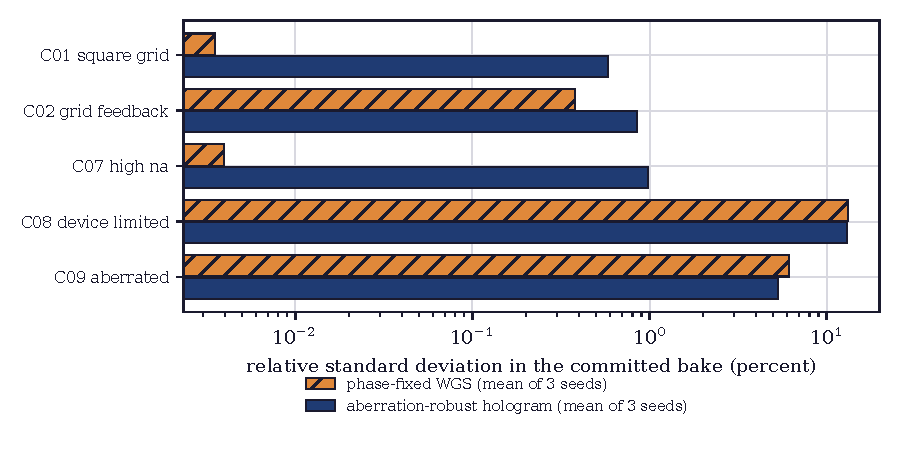
\includegraphics[width=0.78\textwidth]{fig-bake.pdf}
\caption{Relative standard deviation of the trap intensities (percent, logarithmic axis) of phase-fixed WGS and of the robust hologram on the five cases of the committed bake that include the robust hologram; mean of three seeds per case, each case with its own optics.}
\label{fig:bake}
\end{figure}

\subsection{Ensembles that differ from the design prior}

Table~\ref{tab:mismatch} and Fig.~\ref{fig:mismatch} score the same holograms, designed for eight modes at \parAb{} waves, on ensembles that differ from the prior: the same standard-normal draws scaled to other amplitudes, and ensembles with additional modes (Noll 12 to 15, and Noll 12 to 21) that the design did not include. For amplitudes below the design the ratio is \misBMed{} at 0.01 waves per mode, above the criterion, and \misAMed{} at 0.005, just below it; the ratio is limited at the lowest amplitude by the nominal spread of the robust hologram, about \thSigmaZeroBfour{} percent against \thSigmaZeroNom{} percent for the baseline. Above the design amplitude the gain falls to
\misDMed{} at 0.03 and \misEMed{} at 0.04 waves per mode. With modes outside the design the ratio is \misFMed{} when four more modes are added and \misGMed{} when the whole set up to Noll 21 is present: the design does nothing for modes it did not see. H7 therefore holds for smaller amplitudes and fails for larger ones and for other modes. The robust hologram is robust to the distribution it was designed for, and a measured residual that differs needs its own prior.

\begin{table}[t]
\centering\small
\caption{Holograms of seeds 1 to 3 on ensembles that differ from the design prior of 0.02 waves per mode over Noll 4 to 11: the 95th percentile of the spread (percent) of phase-fixed WGS and of the robust hologram (medians), the ratio with the range over the seeds, and the efficiency ratio.}
\label{tab:mismatch}
\begin{tabular}{@{}l r r l r@{}}
\toprule
Evaluation ensemble & $Q_{95}$ WGS & $Q_{95}$ robust & $\rho$ (range) & $\eta$\\
\midrule
0.005 waves per mode, Noll 4 to 11 & 1.42 & 1.13 & 1.24 (1.22 to 1.34) & 0.981 \\
0.01 waves per mode, Noll 4 to 11 & 2.85 & 1.65 & 1.75 (1.72 to 1.77) & 0.981 \\
0.02 waves per mode, Noll 4 to 11 & 6.07 & 4.22 & 1.43 (1.42 to 1.57) & 0.982 \\
0.03 waves per mode, Noll 4 to 11 & 10.01 & 8.60 & 1.16 (1.06 to 1.20) & 0.983 \\
0.04 waves per mode, Noll 4 to 11 & 15.17 & 14.82 & 1.02 (0.99 to 1.03) & 0.985 \\
design modes plus 12 to 15 added & 6.64 & 5.40 & 1.22 (1.19 to 1.24) & 0.983 \\
design modes plus Noll 12 to 21 & 10.66 & 10.63 & 0.99 (0.97 to 1.02) & 0.984
\\
\bottomrule
\end{tabular}
\end{table}

\begin{figure}[t]
\centering
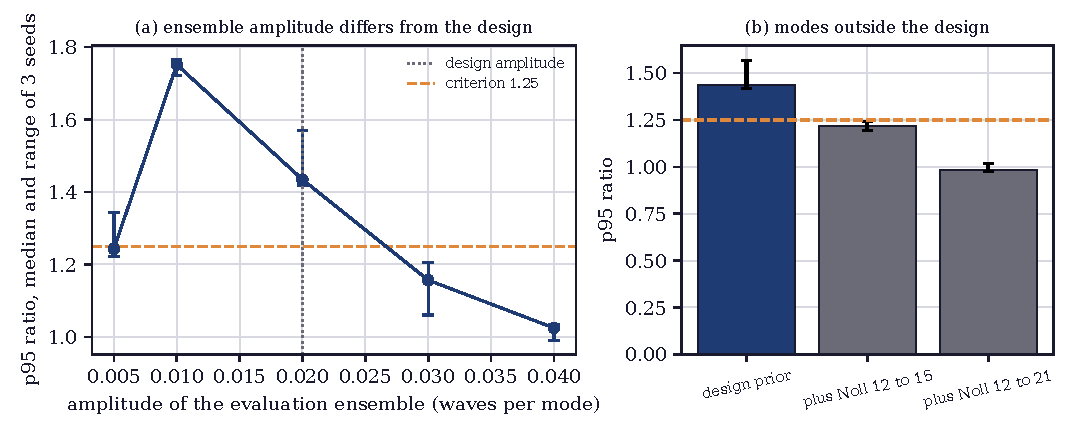
\includegraphics[width=\textwidth]{fig-mismatch.pdf}
\caption{(a) Ratio of the 95th percentiles against the amplitude of the evaluation ensemble, for holograms designed at 0.02 waves per mode; median and range of three seeds. (b) The same ratio on the design prior and on ensembles that add Noll modes 12 to 15 and 12 to 21 at 0.02 waves per mode.}
\label{fig:mismatch}
\end{figure}

\subsection{Check of the first-order theory}

Table~\ref{tab:theory} and Fig.~\ref{fig:theory} test Proposition 3 on the three seeds. The first-order response matrix $G$ was computed by central differences of $\pm10^{-3}$ waves in each of the eight modes at the nominal system, and the spread of each of the 200 draws was predicted from it. For phase-fixed WGS the prediction follows the draws closely: the Pearson correlation between the predicted and the measured spread is \thPearsonNom, the predicted mean squared spread is \thPredSqNom{} against \thMeasSqNom{} measured, and the 95th percentile is \thQLinNom{} against \thQMeasNom{} percent. For the robust hologram the correlation is
\thPearsonBfour, the predicted mean squared spread is \thPredSqBfour{} against \thMeasSqBfour{} measured, and the predicted 95th percentile is \thQLinBfour{} against \thQMeasBfour{}. H5 is met for the baseline and not for the robust hologram, by either of its two parts: the correlation is below $0.9$ and the measured mean squared spread exceeds the first-order value on both holograms (the first-order value is an approximation and not a strict bound, since it neglects the second-order terms of the response).
The first-order intensity variance $s^2\sum G^2$ falls by a factor of \thPRatio{} from the baseline to the robust hologram, so the first-order model predicts a ratio of 95th percentiles of about \thQLinRatio{} where the measurement gives \ratioMed. The optimizer removes most of the first-order response, and the spread that remains in the ensemble is mostly second order in the aberration, which the sigma points reach only through the second derivatives (Proposition 1).

\begin{table}[t]
\centering\small
\caption{Check of the first-order model of the spread (Proposition 3) for each seed and hologram: nominal spread $\sigma_0$ (percent), measured mean squared spread over the 200 draws, the value $\sigma_0^2+s^2\operatorname{tr}\Gamma$, the uncentred bound of Eq.~\eqref{eq:spreadbound}, the Pearson correlation between predicted and measured spread per draw, and the measured and predicted 95th percentiles (percent).}
\label{tab:theory}
\small
\begin{tabular}{@{}r l r r r r r r r@{}}
\toprule
Seed & Hologram & $\sigma_0$ & measured $\overline{\sigma^2}$ & first order & bound & Pearson & $Q_{95}$ & $Q_{95}$ first order\\
\midrule
1 & phase-fixed WGS & 0.0093 & 15.88 & 14.78 & 14.78 & 0.983 & 6.19 & 5.82 \\
1 & B4 & 0.88 & 5.78 & 4.11 & 4.11 & 0.897 & 3.95 & 2.89 \\
2 & phase-fixed WGS & 0.37 & 14.87 & 13.59 & 13.59 & 0.978 & 5.98 & 5.68 \\
2 & B4 & 1 & 5.39 & 3.73 & 3.74 & 0.877 & 4.22 & 2.68 \\
3 & phase-fixed WGS & 0.015 & 14.86 & 13.40 & 13.40 & 0.974 & 6.07 & 5.70 \\
3 & B4 & 1 & 5.66 & 3.81 & 3.82 & 0.867 & 4.23 & 2.79
\\
\bottomrule
\end{tabular}
\end{table}

Table~\ref{tab:cost} decomposes the robust cost of Proposition 2 at the level $\ell=\parLevel$. The nominal cost $L_0$ of the baseline is \thLzeroNom, the sigma-point average $J_{\mathcal S}$ is \thJsigNom, and the difference $J_{\mathcal S}-L_0$ is \thDeltaJNom, negative; the Gauss--Newton term is \thGNNom, positive and small, so the residual term of Eq.~\eqref{eq:curvature} is the large one, of size \thResidNom. The reason is that the level is a fraction of the start efficiency: aberrations lower the mean intensity of the traps toward the target (the start efficiency is
\startEffOne{} and the mean efficiency over the ensemble is \effDropOne{} of it, close to the exponential approximation of the Strehl ratio, \strehlExp), so the expected cost of the baseline is lower than its nominal cost. The level of $\ell=\parLevel$ thus encodes the expected loss of mean intensity, which is why the ablation of the level in Section~\ref{sec:ablation} has its maximum there, and the robust cost lowers $J_{\mathcal S}$ further, to \thJsigBfour{} for the robust hologram.

\begin{figure}[t]
\centering
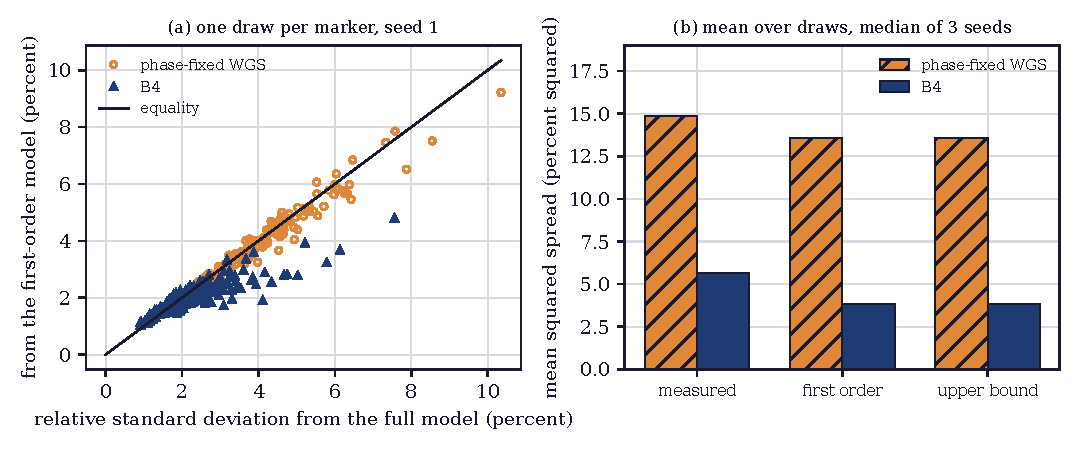
\includegraphics[width=\textwidth]{fig-theory.pdf}
\caption{(a) Relative standard deviation of each of the 200 draws predicted by the first-order model of the response against the value computed with the full model, for phase-fixed WGS and the robust hologram (seed 1). (b) Mean squared relative standard deviation over the draws: measured, first-order value and uncentred bound, median of three seeds.}
\label{fig:theory}
\end{figure}

\begin{table}[t]
\centering\small
\caption{Decomposition of the expected cost for each seed and hologram at the level used by the robust hologram: nominal cost $L_0$, sigma-point average $J_{\mathcal S}$, their difference, and the Gauss--Newton term $s^2\sum G^2/T_\Sigma$ of Eq.~\eqref{eq:curvature}.}
\label{tab:cost}
\begin{tabular}{@{}r l r r r r@{}}
\toprule
Seed & Hologram & $L_0$ & $J_{\mathcal S}$ & $J_{\mathcal S}-L_0$ & Gauss--Newton\\
\midrule
1 & phase-fixed WGS & 0.0123 & 0.00194 & $-$0.0104 & 0.00183 \\
1 & robust hologram & 0.00799 & 0.000743 & $-$0.00724 & 0.000395 \\
2 & phase-fixed WGS & 0.0124 & 0.00185 & $-$0.0105 & 0.00166 \\
2 & robust hologram & 0.00828 & 0.000656 & $-$0.00762 & 0.000317 \\
3 & phase-fixed WGS & 0.0123 & 0.00184 & $-$0.0105 & 0.00165 \\
3 & robust hologram & 0.00824 & 0.000669 & $-$0.00758 & 0.000336
\\
\bottomrule
\end{tabular}
\end{table}

\subsection{Pointing errors}

The acceptance configuration of the method for random displacements of the traps, 3 steps of 2 draws and a displacement of $0.15$ focal bins, is scored on a joint ensemble of aberrations and displacements (the aberration of the design prior is present in both). Table~\ref{tab:pointing} gives the 95th percentiles of the baseline and of the robust hologram: on seed 1 they are \ptAccNomOne{} and \ptAccBfourOne{} percent, a ratio of \ptAccOne, and over the three seeds the ratio has a median of \ptAccMed{}
and a range from \ptAccMin{} to \ptAccMax, below the criterion, and below one on one seed. With 20 steps of the sample design and a displacement prior of 0.05, 0.10 and 0.15 bins, the median ratios are \ptASample{}, \ptBSample{} and \ptCSample. The hologram of the aberration design, released as the method, scores \ptASigma, \ptBSigma{} and \ptCSigma{} on the same joint ensembles, higher because the aberration part of the joint ensemble is the part it was designed for.

\begin{table}[t]
\centering\small
\caption{Pointing errors on the joint ensemble of aberrations and displacements: 95th percentile of the spread (percent) of phase-fixed WGS and of the sample design, and their ratio, for the acceptance configuration (3 steps, 2 draws, 0.15 bin, 20 ensemble draws) and for 20 steps of 8 draws at three displacements (100 ensemble draws).}
\label{tab:pointing}
\begin{tabular}{@{}r l r r r@{}}
\toprule
Seed & Configuration & $Q_{95}$ WGS & $Q_{95}$ robust & $\rho$\\
\midrule
1 & acceptance configuration, 0.15 bin, 20 draws & 8.492 & 8.152 & 1.04 \\
1 & 20 steps, 8 draws per step, 0.05 bin, 100 draws & 6.380 & 6.014 & 1.06 \\
1 & 20 steps, 8 draws per step, 0.10 bin, 100 draws & 6.858 & 6.551 & 1.05 \\
1 & 20 steps, 8 draws per step, 0.15 bin, 100 draws & 7.618 & 7.440 & 1.02 \\
2 & acceptance configuration, 0.15 bin, 20 draws & 7.475 & 7.129 & 1.05 \\
2 & 20 steps, 8 draws per step, 0.05 bin, 100 draws & 6.261 & 5.611 & 1.12 \\
2 & 20 steps, 8 draws per step, 0.10 bin, 100 draws & 6.840 & 6.313 & 1.08 \\
2 & 20 steps, 8 draws per step, 0.15 bin, 100 draws & 7.617 & 7.496 & 1.02 \\
3 & acceptance configuration, 0.15 bin, 20 draws & 7.454 & 8.732 & 0.85 \\
3 & 20 steps, 8 draws per step, 0.05 bin, 100 draws & 6.423 & 6.045 & 1.06 \\
3 & 20 steps, 8 draws per step, 0.10 bin, 100 draws & 6.827 & 6.404 & 1.07 \\
3 & 20 steps, 8 draws per step, 0.15 bin, 100 draws & 7.413 & 7.189 & 1.03
\\
\bottomrule
\end{tabular}
\end{table}

To separate the effects, the aberration was removed from both the design and the ensemble, leaving displacements alone (Table~\ref{tab:pointonly}). The mean spread of the baseline is \poANom{}, \poBNom{} and \poCNom{} percent at displacements of 0.05, 0.10 and 0.15 bins, which is far above what the curvature of Proposition 4 alone predicts, \poAPred{}, \poBPred{} and \poCPred{} percent (the curvature, measured by finite differences, is \poKx{} per bin squared along $x$ and \poKy{} along $y$, within
a few percent of the value \curvAp{} computed from the beam, and the robust hologram has \curvBfour). The spread is dominated by a first-order term: the mean square slope of the trap intensity with the displacement is \poSlopeSq{} per bin squared (rms \poSlopeRms{} per bin), and Eq.~\eqref{eq:pointing} with the measured slope and curvature gives \poAPredSlope{}, \poBPredSlope{} and \poCPredSlope{} percent, within about five percent of the measured values. The curvature of Proposition 4 fixes the second-order floor, and not the spread
that is measured at these displacements. Figure~\ref{fig:pointing} summarizes the ratios of all the configurations and the curvature.

A displacement prior alone, with 20 steps of Adam and 8 draws, gives ratios of 95th percentiles of \poARatio, \poBRatio{} and \poCRatio{} at 0.05, 0.10 and 0.15 bins (medians over three seeds; the range at 0.05 bins is \poARatioMin{} to \poARatioMax). With five times the budget (100 steps) the ratios are \poALong{} (\poALongMin{} to \poALongMax), \poBLong{} (\poBLongMin{} to \poBLongMax) and \poCLong{} (\poCLongMin{} to \poCLongMax), at efficiency ratios of \poALongEff, \poBLongEff{} and \poCLongEff,
and the mean square slope falls from \poSlopeSq{} to \poBLongSlope{} per bin squared at 0.10 bins while the curvature stays at \poBLongCurv. The measured spread at 0.10 bins is then \poBLongMean{} percent, about 30 percent above the curvature floor of \poBPred{} percent that the model of Proposition 4 gives, and the gain costs efficiency: the ratio at 0.05 bins is the smallest and its efficiency ratio is \poALongEff. H6 is refuted in the configuration of the acceptance test and in the 20-step design with the aberration prior, and it is not refuted when the displacement prior is optimized alone for 100 steps at the larger displacements; the budget decides, and what remains is the curvature floor that Proposition 4 describes.

\begin{table}[t]
\centering\small
\caption{Displacements alone (no aberration in the design or the ensemble), medians over seeds 1 to 3 are in the text; per seed and displacement: mean spread over 200 draws of phase-fixed WGS (percent), the value predicted from the curvature alone and from the slope and the curvature, the mean spread of the aberration design, of a displacement-only design with 20 steps, and the 95th percentiles of the baseline, of the 20-step design and of the 100-step design.}
\label{tab:pointonly}
\small
\begin{tabular}{@{}r r r r r r r r r r@{}}
\toprule
Seed & bins & WGS & curv. & slope & B4 & 20 st. & $Q_{95}$ WGS & $Q_{95}$ 20 st. & $Q_{95}$ 100 st.\\
\midrule
1 & 0.05 & 1.09 & 0.31 & 1.11 & 1.41 & 1.65 & 1.29 & 1.85 & 1.26 \\
1 & 0.10 & 2.40 & 1.23 & 2.46 & 2.58 & 2.57 & 2.86 & 3.05 & 1.99 \\
1 & 0.15 & 4.06 & 2.77 & 4.23 & 4.19 & 3.90 & 4.99 & 4.83 & 3.48 \\
2 & 0.05 & 1.09 & 0.31 & 1.05 & 1.50 & 1.42 & 1.29 & 1.59 & 1.04 \\
2 & 0.10 & 2.31 & 1.23 & 2.35 & 2.61 & 2.35 & 2.77 & 2.74 & 1.84 \\
2 & 0.15 & 3.93 & 2.77 & 4.09 & 4.19 & 3.71 & 4.73 & 4.41 & 3.47 \\
3 & 0.05 & 1.05 & 0.31 & 1.06 & 1.49 & 1.52 & 1.25 & 1.69 & 1.13 \\
3 & 0.10 & 2.33 & 1.23 & 2.38 & 2.62 & 2.45 & 2.85 & 2.81 & 1.93 \\
3 & 0.15 & 3.98 & 2.77 & 4.12 & 4.22 & 3.82 & 4.85 & 4.53 & 3.53
\\
\bottomrule
\end{tabular}
\end{table}

\begin{figure}[t]
\centering
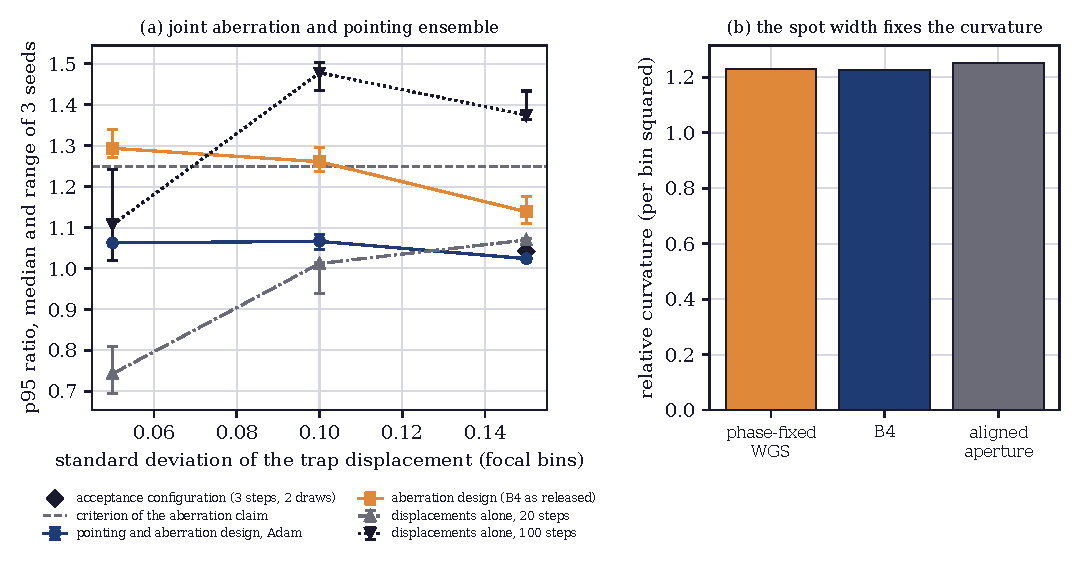
\includegraphics[width=\textwidth]{fig-pointing.pdf}
\caption{(a) Ratio of the 95th percentiles against the displacement for the joint ensemble (sample design and aberration design) and for displacements alone (20 and 100 steps); median and range of three seeds, with the acceptance configuration as a diamond. (b) Relative curvature of the trap intensity under displacement for phase-fixed WGS, the robust hologram and the aligned-aperture value of Proposition 4.}
\label{fig:pointing}
\end{figure}

\section{Ablation}\label{sec:ablation}

\subsection{What each element contributes}

Table~\ref{tab:abl} gives the ratio $\rho$ of the 95th percentiles and the efficiency ratio $\eta$ of each variant of the method, as the median over seeds 1 to 3 with the range of $\rho$; Fig.~\ref{fig:ablation} shows the ratios. Every variant is scored on the acceptance ensemble against the phase-fixed WGS hologram of its own seed, and differs from the method in one element.
The rows are read in groups.

\emph{Design samples.} Minimizing the nominal cost with the same solver, budget, level and start (one design point at the origin) does not lower the spread: $\rho=\ablNominalMed$ (\ablNominalMin{} to \ablNominalMax) at $\eta=\ablNominalEff$, so the gain is not the work of the extra iterations, and a hologram pushed toward a level of $0.9$ of its own efficiency without the aberration terms is worse than the starting one. Random draws held fixed during the descent
recover part of the gain, and the gain grows with their number: $\rho$ is \ablRandFourMed{} for 4 draws, \ablRandEightMed{} for 8, \ablRandSixteenMed{} for 16 and \ablRandThirtyTwoMed{} for 32. The 16 sigma points reach \ablDefaultMed{}, above the range of 16 random draws (up to \ablRandSixteenMax) and above the median of 32. Resampling 8 random draws at every step with Adam gives \ablAdamMed{} (\ablAdamMin{} to \ablAdamMax) at the highest
efficiency of the group, $\eta=\ablAdamEff$. H4 holds: for the same number of design samples the deterministic set gives the larger ratio, and the deterministic set also costs the fewest evaluations of the cost for the ratio it reaches.

\emph{Modes in the design.} A design that covers part of the modes of the ensemble does not protect against the rest. With defocus only $\rho$ is \ablModesDefocusMed, with Noll 4 to 6 \ablModesToSixMed, with Noll 4 to 8 \ablModesToEightMed, and a design on Noll 9 to 11, which are not the modes that dominate the ensemble spread, gives \ablModesHighMed; only the full set of eight reaches \ablDefaultMed. An incomplete design is worse than the baseline on the full ensemble; the measurement does not isolate the mechanism, and the result is the reason the designed modes must cover the modes of the residual.

\emph{Design amplitude.} The design amplitude has a sharp optimum at the amplitude of the ensemble, $0.02$ waves per mode: $\rho$ is \ablPriorAMed{} at 0.005, \ablPriorBMed{} at 0.01, \ablDefaultMed{} at 0.02, \ablPriorDMed{} at 0.03 and \ablPriorEMed{} at 0.04. The target level was held at \parLevel{} in all of these, and the level is tied to the amplitude by the Strehl ratio (Section~\ref{sec:results}), so a change of the amplitude alone moves the design off its best level; the
ablation varies one element at a time and does not map the pair.

\subsection{Level and iterations}

Figure~\ref{fig:level} plots the trade-off of the level. A level of $0.80$ lowers the efficiency to \ablLevelAEff{} of the baseline and the ratio to \ablLevelAMed; levels of $0.85$, $0.90$, $0.937$, $0.95$ and $1.00$ give \ablLevelBMed, \ablDefaultMed, \ablLevelDMed, \ablLevelEMed{} and \ablLevelFMed{} at efficiency ratios of \ablLevelBEff, \ablDefaultEff, \ablLevelDEff, \ablLevelEEff{} and \ablLevelFEff. The ratio is highest at the level of
$0.90$, near the Strehl ratio of the ensemble (\strehlExp), and falls on both sides; higher levels return the efficiency to or above that of the baseline (the efficiency ratio is above one from $0.937$ on) and give up part of the gain, so the level is the dial between efficiency and robustness. A user who needs to keep the full efficiency of phase-fixed WGS can take $\ell=0.937$, which keeps $\eta\ge1$ at a ratio of \ablLevelDMed.

\begin{table}[t]
\centering\small
\caption{Ablation on seeds 1 to 3 against the acceptance ensemble: ratio $\rho$ of the 95th percentiles of phase-fixed WGS and of each variant (median and range over seeds) and efficiency ratio $\eta$ (median). The variants differ from the method in one element: the design samples, the modes in the design, the design amplitude, the target level and the number of conjugate-gradient iterations.}
\label{tab:abl}
\begin{tabular}{@{}l r l r@{}}
\toprule
Variant & $\rho$ (median) & range & $\eta$\\
\midrule
\emph{Design samples} & & & \\
\quad sigma points, 16 deterministic draws (B4) & 1.43 & 1.42 to 1.57 & 0.982 \\
\quad nominal cost only, same CG (one point) & 0.62 & 0.56 to 0.71 & 0.891 \\
\quad 4 fixed random draws, same CG & 1.00 & 0.98 to 1.12 & 0.952 \\
\quad 8 fixed random draws, same CG & 1.20 & 1.12 to 1.21 & 0.972 \\
\quad 16 fixed random draws, same CG & 1.33 & 1.26 to 1.36 & 0.974 \\
\quad 32 fixed random draws, same CG & 1.39 & 1.33 to 1.44 & 0.980 \\
\quad resampled draws (8 per step), Adam & 1.24 & 1.16 to 1.28 & 0.988 \\
\midrule
\emph{Modes in the design} & & & \\
\quad defocus only (Noll 4) & 0.75 & 0.59 to 0.82 & 0.901 \\
\quad Noll 4 to 6 & 0.92 & 0.70 to 0.92 & 0.924 \\
\quad Noll 4 to 8 & 1.17 & 1.13 to 1.17 & 0.952 \\
\quad Noll 9 to 11 (not the dominant modes) & 0.89 & 0.75 to 0.94 & 0.924 \\
\quad Noll 4 to 11 (B4) & 1.43 & 1.42 to 1.57 & 0.982 \\
\midrule
\emph{Design amplitude} & & & \\
\quad design amplitude 0.005 waves per mode & 0.65 & 0.60 to 0.75 & 0.898 \\
\quad design amplitude 0.01 waves per mode & 0.84 & 0.83 to 0.87 & 0.916 \\
\quad design amplitude 0.02 waves per mode (B4) & 1.43 & 1.42 to 1.57 & 0.982 \\
\quad design amplitude 0.03 waves per mode & 1.13 & 1.07 to 1.23 & 1.012 \\
\quad design amplitude 0.04 waves per mode & 0.90 & 0.90 to 0.98 & 1.016 \\
\midrule
\emph{Target level} & & & \\
\quad target level 0.80 & 0.71 & 0.53 to 0.78 & 0.849 \\
\quad target level 0.85 & 1.25 & 1.04 to 1.29 & 0.929 \\
\quad target level 0.90 (B4) & 1.43 & 1.42 to 1.57 & 0.982 \\
\quad target level 0.937 & 1.27 & 1.24 to 1.33 & 1.006 \\
\quad target level 0.95 & 1.19 & 1.18 to 1.26 & 1.009 \\
\quad target level 1.00 & 1.06 & 1.04 to 1.14 & 1.014 \\
\midrule
\emph{Iterations} & & & \\
\quad 5 CG iterations & 1.30 & 1.28 to 1.36 & 0.981 \\
\quad 10 CG iterations & 1.33 & 1.27 to 1.37 & 0.978 \\
\quad 20 CG iterations & 1.40 & 1.39 to 1.53 & 0.981 \\
\quad 40 CG iterations (B4) & 1.43 & 1.42 to 1.57 & 0.982 \\
\quad 80 CG iterations & 1.44 & 1.42 to 1.56 & 0.984
\\
\bottomrule
\end{tabular}
\end{table}

\begin{figure}[t]
\centering
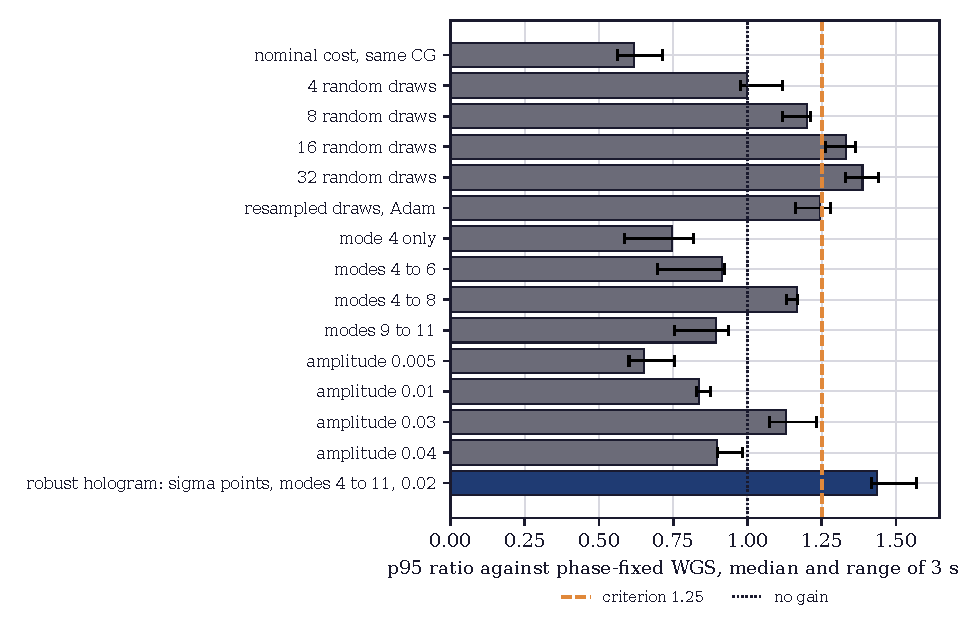
\includegraphics[width=0.8\textwidth]{fig-ablation.pdf}
\caption{Ratio of the 95th percentiles against phase-fixed WGS for each variant of the design samples, the modes and the design amplitude, median and range over three seeds, with the full method as the dark bar; the dashed line is the criterion of 1.25 and the dotted line marks no gain.}
\label{fig:ablation}
\end{figure}

\begin{figure}[t]
\centering
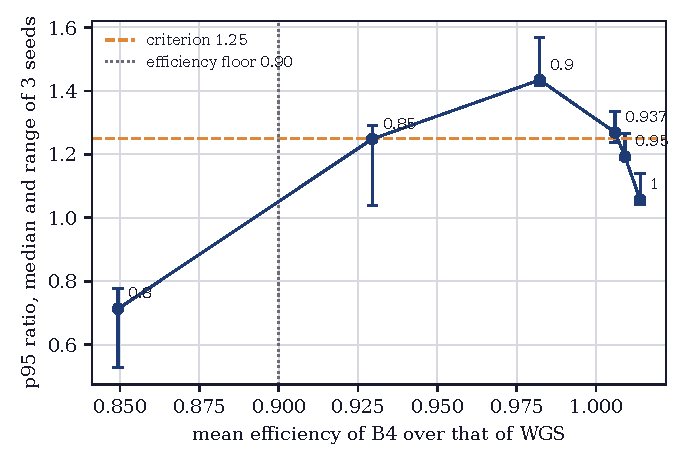
\includegraphics[width=0.62\textwidth]{fig-level.pdf}
\caption{Trade-off of the target level: ratio of the 95th percentiles against the efficiency ratio for target levels from 0.80 to 1.00 (labels), median and range of three seeds; the dashed line is the criterion of 1.25 and the dotted line the efficiency floor of 0.90.}
\label{fig:level}
\end{figure}

The iterations (Fig.~\ref{fig:conv}) matter little beyond the first few: the ratio is \ablIterAMed{} after 5 iterations, \ablIterBMed{} after 10, \ablIterCMed{} after 20, \ablDefaultMed{} after 40 and \ablIterEMed{} after 80, all at $\eta\approx0.98$. The expected cost falls from \lossStart{} to \lossEnd{} over the 40 iterations of seed 1, most of it in the first iterations. The method is cheap to stop early: five iterations already exceed the criterion on every seed.

\begin{figure}[t]
\centering
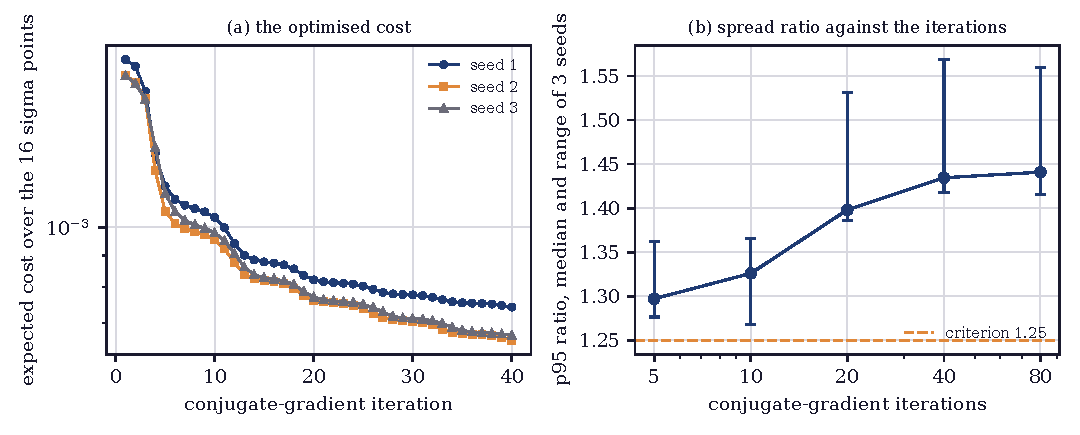
\includegraphics[width=\textwidth]{fig-conv.pdf}
\caption{(a) Expected cost over the 16 sigma points along the 40 conjugate-gradient iterations for seeds 1 to 3 (logarithmic axis). (b) Ratio of the 95th percentiles against the number of iterations, median and range of three seeds, with the criterion of 1.25.}
\label{fig:conv}
\end{figure}

\section{Discussion}\label{sec:discussion}

\subsection{Where the gain comes from}

Three pieces of evidence locate the gain. First, the control of the ablation: the same solver and budget on the nominal cost does not lower the spread (a ratio of \ablNominalMed), so the expected cost is the cause and the extra iterations are not. Second, the theory check: the first-order intensity variance induced by the aberration prior falls by a factor of \thPRatio{} from phase-fixed WGS to the robust hologram, the first-order model follows the draws of the baseline with a correlation of \thPearsonNom, and the robust hologram has \thSigmaZeroBfour{} percent nominal spread against \thSigmaZeroNom{} for the baseline, the price of the flatter response.
Third, the draws: the robust hologram has the lower spread on every draw of seed 1, which is what a lower response would produce and what a lucky tail would not.

The first-order model also says what the method does not do. It predicts a ratio of the 95th percentiles of about \thQLinRatio{} and the measurement gives \ratioMed. The difference is the second-order part of the response, which the design reaches only through the second derivatives of the cost that the sigma points match, and which grows with the aberration: at a Strehl ratio of about \strehlExp{} the rms phase offset is \phaseRms{} rad, and the first-order model of the robust hologram under-predicts its own mean squared spread by about a third
(\thPredSqBfour{} against \thMeasSqBfour). The gain is real and smaller than the first-order theory suggests. A design that reduced the second-order response directly, for example by including the quadratic terms of the intensity in the cost, is a candidate extension that this paper does not test.

\subsection{The level and the Strehl ratio}

The decomposition of the cost shows a second mechanism that Proposition 2 alone does not predict. At a target level of $0.90$ of the start efficiency, the expected cost of the baseline is lower than its nominal cost, because the aberrations lower the mean intensity of the traps (to \effDropOne{} of the start efficiency in the ensemble) toward the target. The level in effect encodes the mean intensity loss that the prior implies, and the ablation of the level has its maximum at the level
that matches the Strehl ratio of the ensemble. This is consistent with the sensitivity of the method to the pair of the design amplitude and the level: a prior of 0.03 waves per mode has a Strehl ratio near \strehlThree{} and wants a lower level, and the ablation of the amplitude at the fixed level of $0.90$ is therefore a conservative test of the amplitude and an unfair test of the level. A study that maps the pair is open. For a user, the consequence is that the level should be set from the measured Strehl ratio of
the residual, and not left at its default.

\subsection{Failure cases and negative results}

Four results are negative or partial. (i) The gain does not transfer to ensembles outside the design: it is \misDMed{} at 0.03 and \misEMed{} at 0.04 waves per mode, and \misGMed{} when modes up to Noll 21 are present. The robust hologram trades breadth for depth over the modes and amplitude it was given. (ii) The nominal spread rises: on the cases without aberration the robust hologram has 0.4 to 1.0 percent spread where the baseline is below 0.01 percent in most seeds, and its mean efficiency is \effRatioMed{} of the baseline's.
An array that needs the lowest nominal spread, and has no residual aberration, should not use it. (iii) For random displacements of the traps, the configuration of the acceptance test gives no gain, and the spread under displacement has a first-order slope term that the curvature of the spot does not explain. The explanation that the spot width alone bounds pointing robustness is incomplete in this model: with a displacement prior alone and enough steps the slope falls fivefold and the ratio reaches \poBLong{} at 0.10 bins at \poBLongEff{} of the baseline's efficiency; what remains is close to the curvature floor.
(iv) The first-order theory is met by the baseline and not by the robust hologram, as above.

\subsection{Relation to the practice of correction and calibration}

The method does not replace the Zernike correction of the large arrays~\cite{nogrette2014,ebadi2021,manetsch2025}; it assumes it. The correction removes the measured wavefront and the method designs for the residual that the correction leaves, with a prior that must come from the instrument. The residual of a real instrument is spatially varying~\cite{machu2025,christen2025}; the isotropic Gaussian prior over eight global modes used here is the simplest description, and a per-site or per-patch residual would give a prior per trap, which the expected-cost formulation accommodates (each sigma point would shift the phase of the traps of a patch) and this paper does not test.
It also does not replace camera feedback~\cite{nogrette2014,kim2019}: feedback corrects the intensities of one realization after the fact, while the expected-cost design lowers the spread of the family of realizations the experiment may present, between recalibrations. The two address different time scales and could be combined, which is a question for an experiment on hardware.

\subsection{What the result supports}

The result supports a limited statement: in a scalar Fourier model with an ideal device, for an array of 100 equal traps, and an aberration residual that is independent, Gaussian and of the amplitude that the design assumes, an expected-cost hologram started from phase-fixed WGS has a 95th-percentile spread about \ratioMed{} times lower at \effRatioMed{} of the efficiency, and a deterministic sigma-point set reaches it with half the evaluations of the 32 random draws that come close. It does not support a claim about hardware, about arrays of thousands of traps, about measured residuals, or about robustness to displacements of the traps in the acceptance configuration. The measured scope is also narrow in the choices that the ablation exposes: the design amplitude, the target level and the designed modes were set to the values of the ensemble, and the table of the ablation shows how quickly the ratio falls when any of them is set to another value. A user who adopts the method owes the same measurement for the instrument at hand: the residual of the correction, its modes and its amplitude, and a scan of the level around the Strehl ratio that the residual implies.

\section{Limitations}\label{sec:limits}

\subsection{Threats to internal validity}

The robust hologram and the baseline are computed by the same engine, from the same random start of each seed, and scored by the same function on the same draws, so the comparison does not depend on a difference of implementation. The ablation uses a replica of the sigma-point loop that takes the design samples as an argument; the replica reproduces the module's hologram on the default configuration to \replicaDiff{} rad, and the evaluator of this paper reproduces the module's ensemble statistics to \evalCheckMax. The seeds are few: three seeds feed every part but the main comparison, so
the ranges of the ablation are ranges over three holograms and not confidence intervals, and a difference between two variants of less than the range is not a result. The bootstrap interval of a single seed measures the finite ensemble, and it is wide (\ciBelowN{} of \nSeedsAll{} intervals reach below the criterion). The ensemble seed of the acceptance test is one draw of 200; the five other ensembles of the held-out test give higher ratios, which suggests that the acceptance ensemble is not favourable but does not bound the variation of
the ensemble. The conjugate-gradient iterations end at a budget and not at a convergence criterion, and the optimizer is not a global one, so the holograms are those of one descent from one start. The first-order model that checks the theory uses finite differences of $10^{-3}$ waves, which is small against the phase offsets of the ensemble but not an analytical derivative.

\subsection{Threats to external validity}

The result is a simulation in a scalar Fourier model with an ideal device: no pixel crosstalk, no phase quantization, no fill factor, no flicker, no camera. The ablation of the design shows that the gain is tied to the match between the design prior and the ensemble in amplitude and in modes, and the ensemble here is drawn from the prior that the design assumes. A real residual is neither independent across modes nor Gaussian nor of one scale, varies across the field, and is a quantity that has to be measured; with the evaluation amplitude $1.5$ times the design amplitude the measured ratio is \misDMed{}, and with the design amplitude $1.5$ times the evaluation amplitude it is \ablPriorDMed. The array is 100 traps on 256 by 256 pixels, a small array compared with the arrays that motivate the work (about a thousand tweezers for the 256-atom machine~\cite{ebadi2021} and about twelve thousand sites for the 6,100-atom array~\cite{manetsch2025}); the cost of a run grows with the pixel count and the trap count (Section~\ref{sec:proposed-method}), and the benefit at that scale is not measured. The traps have equal weights, and the first-order
theory is stated for that case. The aberration enters as a phase offset on the SLM plane, as in the sources, and a field-dependent aberration, for which each trap sees a different wavefront, is not modelled.

\subsection{Threats to construct validity}

The spread $\sigma$ is the relative standard deviation of the trap intensities across one realization, and the 95th percentile is taken over realizations. The quantity that an experiment needs may be the trap depth of each site, its stability over time, or the loading probability, which depend on the intensity through physics outside this model; the spread of the intensities is a proxy. The efficiency counts the light in the traps and not the light in the zero order or in ghost spots. The ratio $\rho$ compares two 95th percentiles of 200 draws each, and
the 95th percentile of such a sample is a noisy statistic, which the bootstrap interval measures for one seed. The 100 traps of equal weight also make the spread a single number per realization; with unequal weights, or traps of different kinds, the construct would have to be defined per class of traps. The claim of the hypotheses H1 and H2 uses the thresholds of the product's acceptance test, and the thresholds are conventions, not requirements of an experiment.

\subsection{Scope}

The method applies to trap targets of point traps in two dimensions; a shaped field is refused. The sigma-point design covers aberrations; the displacement prior needs the sampled design, which is a different cost with different results, reported in Section~\ref{sec:results}. The method is an offline design: it needs on the order of \runSeconds{} seconds of wall-clock time per hologram in the conditions of the measurement and is not part of a live rearrangement loop. It is not a replacement for aberration correction, camera feedback or a model of the device, and it was not combined with any of them in these experiments. Combined use is plausible, since the correction fixes the nominal system around which the prior is centred and the device model fixes the forward map, but the interaction (a correction with its own error, a prior centred on an estimate, a cost evaluated on a device model with crosstalk) is not measured here and may change the optimum of the level and of the design amplitude.

\section{Reproducibility}\label{sec:repro}

The source code, the engine, the tests and the scripts of this paper are in the repository named in the header block. The method is the module \texttt{data-pipeline/pipeline/model/holo/methods/beyond/b4\_robust.py}, gated by \texttt{tests/methods/beyond/test\_b4\_robust.py}; the acceptance measurement of the same method inside the studio's report is
\texttt{manuscripts/holographic-trap-studio/data/acceptance.py}. No external data are used, so nothing needs to be downloaded: the task, the setup and the ensemble are generated by the portable generator from the seeds stated in Section~\ref{sec:design}, and the cases of the committed bake are read from
\texttt{data-pipeline/pipeline/cases/measured\_ranges.json}.

Every number of the text, every table and every figure is written by a script. From the repository root, with the pipeline environment of the repository, the command
\begin{center}\texttt{python manuscripts/aberration-robust-hologram/data/measure.py --workers \workersUsed{} --seeds \nSeedsAll}\end{center}
runs the measurement (\totalMinutes{} minutes with \workersUsed{} worker processes on the development machine, plus \pointonlyMinutes{} minutes for the pointing-only part) and writes \texttt{data/robust.json}, the macro file \texttt{data/robust\_numbers.tex} that the text reads, and the table files \texttt{data/tab\_*.tex}. The option \texttt{--emit-only} rewrites the macros and the tables from the stored JSON without rerunning the optimizer, and \texttt{--extra pointonly}
reruns the pointing-only measurement on the cached holograms. The command \texttt{python manuscripts/aberration-robust-hologram/figures/make\_figs.py}, with the notebook environment that holds the plotting library, rewrites the eleven vector figures from the JSON. The text is built from \texttt{tex/main.tex} with three passes of \texttt{pdflatex}; the bibliography is in the source.

The runs are deterministic: each method takes its seed through the portable generator (xoshiro128** seeded by SplitMix32), so a rerun gives the same holograms up to the floating point of the machine's fast Fourier transform. The wall-clock times in the text depend on the machine and on the number of processes sharing it; the numbers of the results do not.

\section{Conclusions}\label{sec:conclusions}

Minimizing the expected trap-intensity cost over a Gaussian prior on residual Zernike aberrations, with a deterministic set of sixteen sigma points and a conjugate-gradient descent from phase-fixed WGS, lowers the 95th percentile of the intensity spread of a $10\times10$ array under residual aberrations by a median factor of \ratioMed{} over three seeds (\ratioMin{} to \ratioMax) and \ratioAllMed{} over \nSeedsAll{} seeds (interval \ratioAllCiLo{} to \ratioAllCiHi), at \effRatioMed{} of the efficiency, in a scalar Fourier model with an ideal device. The gain needs the expected cost (the nominal cost with the same solver gives \ablNominalMed), a design that covers the modes of the residual, and a design amplitude and a target level near the ones of the ensemble. It
does not transfer to larger amplitudes or to modes outside the design, and it adds a nominal spread of about one percent. The first-order theory explains the direction of the gain and overstates its size, as the measured ratio is below the first-order prediction of about \thQLinRatio. For random displacements of the traps the acceptance configuration gives a ratio of \ptAccMed{}, and a displacement prior optimized alone for 100 steps gives \poBLong{} at 0.10 bins at \poBLongEff{} of the efficiency; the spread under displacement has a first-order slope term that the design can lower and a curvature floor that the spot width fixes. The next steps are a measurement of the residual of an instrument to give the prior a source, a per-patch prior, a design that includes the second-order response, and a test on hardware.


\begin{thebibliography}{99}\small
\bibitem{ashkin1986} A. Ashkin, J. M. Dziedzic, J. E. Bjorkholm and S. Chu, ``Observation of a single-beam gradient force optical trap for dielectric particles,'' \emph{Opt. Lett.} 11, 288, 1986. doi:10.1364/OL.11.000288.
\bibitem{dileonardo2007} R. Di Leonardo, F. Ianni and G. Ruocco, ``Computer generation of optimal holograms for optical trap arrays,'' \emph{Opt. Express} 15, 1913, 2007. doi:10.1364/OE.15.001913.
\bibitem{polin2005} M. Polin, K. Ladavac, S.-H. Lee, Y. Roichman and D. G. Grier, ``Optimized holographic optical traps,'' \emph{Opt. Express} 13, 5831, 2005. doi:10.1364/OPEX.13.005831.
\bibitem{pasienski2008} M. Pasienski and B. DeMarco, ``A high-accuracy algorithm for designing arbitrary holographic atom traps,'' \emph{Opt. Express} 16, 2176, 2008. doi:10.1364/OE.16.002176.
\bibitem{montes2006} M. Montes-Usategui, E. Pleguezuelos, J. Andilla and E. Mart\'in-Badosa, ``Fast generation of holographic optical tweezers by random mask encoding of Fourier components,'' \emph{Opt. Express} 14, 2101, 2006. doi:10.1364/OE.14.002101.
\bibitem{kim2019} D. Kim, A. Keesling, A. Omran, H. Levine, H. Bernien, M. Greiner, M. D. Lukin and D. R. Englund, ``Large-scale uniform optical focus array generation with a phase spatial light modulator,'' \emph{Opt. Lett.} 44, 3178, 2019. doi:10.1364/OL.44.003178.
\bibitem{kim2019oe} H. Kim, M. Kim, W. Lee and J. Ahn, ``Gerchberg-Saxton algorithm for fast and efficient atom rearrangement in optical tweezer traps,'' \emph{Opt. Express} 27, 2184, 2019. doi:10.1364/OE.27.002184.
\bibitem{harte2014} T. Harte, G. D. Bruce, J. Keeling and D. Cassettari, ``Conjugate gradient minimisation approach to generating holographic traps for ultracold atoms,'' \emph{Opt. Express} 22, 26548, 2014. doi:10.1364/OE.22.026548.
\bibitem{bowman2017} D. Bowman, T. L. Harte, V. Chardonnet, C. De Groot, S. J. Denny, G. Le Goc, M. Anderson, P. Ireland, D. Cassettari and G. D. Bruce, ``High-fidelity phase and amplitude control of phase-only computer generated holograms using conjugate gradient minimisation,'' \emph{Opt. Express} 25, 11692, 2017. doi:10.1364/OE.25.011692.
\bibitem{chakravarthula2019} P. Chakravarthula, Y. Peng, J. Kollin, H. Fuchs and F. Heide, ``Wirtinger holography for near-eye displays,'' \emph{ACM Trans. Graph.} 38, 2019. doi:10.1145/3355089.3356539.
\bibitem{peng2020} Y. Peng, S. Choi, N. Padmanaban and G. Wetzstein, ``Neural holography with camera-in-the-loop training,'' \emph{ACM Trans. Graph.} 39, 2020. doi:10.1145/3414685.3417802.
\bibitem{eybposh2020} M. H. Eybposh, N. W. Caira, M. Atisa, P. Chakravarthula and N. C. P\'egard, ``DeepCGH: 3D computer-generated holography using deep learning,'' \emph{Opt. Express} 28, 26636, 2020. doi:10.1364/OE.399624.
\bibitem{shi2021} L. Shi, B. Li, C. Kim, P. Kellnhofer and W. Matusik, ``Towards real-time photorealistic 3D holography with deep neural networks,'' \emph{Nature} 591, 234--239, 2021. doi:10.1038/s41586-020-03152-0.
\bibitem{whyte2005} G. Whyte and J. Courtial, ``Experimental demonstration of holographic three-dimensional light shaping using a Gerchberg--Saxton algorithm,'' \emph{New J. Phys.} 7, 117, 2005. doi:10.1088/1367-2630/7/1/117.
\bibitem{schroff2023} P. Schroff, A. La Rooij, E. Haller and S. Kuhr, ``Accurate holographic light potentials using pixel crosstalk modelling,'' \emph{Sci. Rep.} 13, 3252, 2023. doi:10.1038/s41598-023-30296-6.
\bibitem{persson2012} M. Persson, D. Engstr\"om and M. Goks\"or, ``Reducing the effect of pixel crosstalk in phase only spatial light modulators,'' \emph{Opt. Express} 20, 22334, 2012. doi:10.1364/OE.20.022334.
\bibitem{nogrette2014} F. Nogrette, H. Labuhn, S. Ravets, D. Barredo, L. B\'eguin, A. Vernier, T. Lahaye and A. Browaeys, ``Single-atom trapping in holographic 2D arrays of microtraps with arbitrary geometries,'' \emph{Phys. Rev. X} 4, 021034, 2014. doi:10.1103/PhysRevX.4.021034.
\bibitem{ebadi2021} S. Ebadi \emph{et al.}, ``Quantum phases of matter on a 256-atom programmable quantum simulator,'' \emph{Nature} 595, 227--232, 2021. doi:10.1038/s41586-021-03582-4.
\bibitem{manetsch2025} H. J. Manetsch, G. Nomura, E. Bataille, X. Lv, K. H. Leung and M. Endres, ``A tweezer array with 6,100 highly coherent atomic qubits,'' \emph{Nature} 647, 60--67, 2025. doi:10.1038/s41586-025-09641-4.
\bibitem{bluvstein2023} D. Bluvstein \emph{et al.}, ``Logical quantum processor based on reconfigurable atom arrays,'' \emph{Nature} 626, 58--65, 2024. doi:10.1038/s41586-023-06927-3.
\bibitem{knottnerus2025} I. H. A. Knottnerus, Y. C. Tseng, A. Urech, R. J. C. Spreeuw and F. Schreck, ``Parallel assembly of neutral atom arrays with an SLM using linear phase interpolation,'' \emph{SciPost Phys.} 19, 118, 2025. doi:10.21468/SciPostPhys.19.4.118.
\bibitem{machu2025} Y. Machu, G. Creutzer, C. Sayrin and M. Brune, ``Full-field-of-view aberration correction for large arrays of focused beams,'' arXiv:2512.15967, 2025. \url{https://arxiv.org/abs/2512.15967}.
\bibitem{christen2025} I. Christen, C. Panuski, T. Propson and D. Englund, ``Full-volume aberration-space holography,'' arXiv:2505.08777, 2025. \url{https://arxiv.org/abs/2505.08777}.
\bibitem{booth2007} M. J. Booth, ``Adaptive optics in microscopy,'' \emph{Phil. Trans. R. Soc. A} 365, 2829--2843, 2007. doi:10.1098/rsta.2007.0013.
\bibitem{jesacher2007} A. Jesacher, A. Schwaighofer, S. F\"urhapter, C. Maurer, S. Bernet and M. Ritsch-Marte, ``Wavefront correction of spatial light modulators using an optical vortex image,'' \emph{Opt. Express} 15, 5801, 2007. doi:10.1364/OE.15.005801.
\bibitem{cizmar2010} T. \v{C}i\v{z}m\'ar, M. Mazilu and K. Dholakia, ``In situ wavefront correction and its application to micromanipulation,'' \emph{Nat. Photonics} 4, 388--394, 2010. doi:10.1038/nphoton.2010.85.
\bibitem{noll1976} R. J. Noll, ``Zernike polynomials and atmospheric turbulence,'' \emph{J. Opt. Soc. Am.} 66, 207, 1976. doi:10.1364/JOSA.66.000207.
\bibitem{mahajan1983} V. N. Mahajan, ``Strehl ratio for primary aberrations in terms of their aberration variance,'' \emph{J. Opt. Soc. Am.} 73, 860, 1983. doi:10.1364/JOSA.73.000860.
\bibitem{julier2004} S. J. Julier and J. K. Uhlmann, ``Unscented filtering and nonlinear estimation,'' \emph{Proc. IEEE} 92, 401--422, 2004. doi:10.1109/JPROC.2003.823141.
\bibitem{fletcher1964} R. Fletcher, ``Function minimization by conjugate gradients,'' \emph{Comput. J.} 7, 149--154, 1964. doi:10.1093/comjnl/7.2.149.
\bibitem{nocedal2006} J. Nocedal and S. J. Wright, \emph{Numerical Optimization}, 2nd ed., Springer, 2006. doi:10.1007/978-0-387-40065-5.
\bibitem{kingma2015} D. P. Kingma and J. Ba, ``Adam: A method for stochastic optimization,'' arXiv:1412.6980, 2014. \url{https://arxiv.org/abs/1412.6980}.
\bibitem{bental2009} A. Ben-Tal, L. El Ghaoui and A. Nemirovski, \emph{Robust Optimization}, Princeton University Press, 2009. doi:10.1515/9781400831050.
\end{thebibliography}


\end{document}
